\documentclass[12pt]{report}
\usepackage[a4paper, left=2cm, right=2cm, top=2.5cm, bottom=2.5cm]{geometry} % Margins
\usepackage{graphicx} % Images
\usepackage{fontspec} % System fonts
\usepackage{hyperref} % Links
\usepackage{minted} % Code
\usepackage{tcolorbox} % Code background
\usepackage{setspace} % Interline spacing
\usepackage{titlesec}
\usepackage{float} % Images H
\usepackage{times}

\definecolor{Titles}{RGB}{100, 25, 104} % Dark blue

\geometry{a4paper, margin=2.5cm}


\titleformat{\chapter}
  {\color{Titles}\normalfont\Huge\bfseries}
  {\thesection}{1em}{}

\titleformat{\section}
  {\color{Titles}\normalfont\LARGE\bfseries}
  {\thesubsection}{1em}{}

  \titleformat{\subsection}
  {\color{Titles}\normalfont\Large\bfseries}
  {\thesubsubsection}{1em}{}
  
\tcbuselibrary{listings, skins, breakable}

\newminted[csharp]{csharp}{ 
    fontsize=\small, 
    fontfamily=tt, 
    bgcolor=black, 
    frame=single, 
    framesep=10pt, 
    rulecolor=\color{white}, 
    breaklines=true, 
    linewidth=100,
    texcl=true,
    style=default,
    keywordstyle=\color{cyan}\bfseries, 
    stringstyle=\color{yellow}, 
    commentstyle=\color{green}, 
    showspaces=false, 
    showstringspaces=false
}

\newtcbox{\code}{
    on line,
    box align=base,
    colback=gray!9,
    colframe=gray!1,
    boxrule=0.4pt,
    arc=4pt,
    top=1pt,
    bottom=0.5pt,
    left=1pt,
    right=1pt,
    fontupper=\ttfamily\fontsize{10}{9}\selectfont,
    nobeforeafter,
}

\setmainfont[
  ItalicFont  = *Italic,
]{Roboto Light} 
\setmonofont[Scale=.9]{Consolas.ttf}[Path=./]

\setlength{\parindent}{0pt}
\setlength{\parskip}{1em}
\onehalfspacing

\title{Messagyre}
\author{TM de Pietro Gravina}

\begin{document}

\maketitle
%\tableofcontents

\chapter{Introduction}

\section{Pourquoi ce sujet}

J’ai choisi de réaliser ce projet car après plus d’un an au Gymnase de Renens, j’ai remarqué l’absence d’un moyen de communication plus informel, malgré la disponibilité de toute la suite Microsoft 365 et d’autres outils. Les e-mails sont trop formels et peu pratiques, tandis que le chat d’Outlook est peu connu et peu intuitif, tout comme celui de Teams.

Pour résoudre ce problème, j’ai conçu une application de messagerie dédiée exclusivement aux communications internes du gymnase : Messagyre. Son principe est similaire à celui de WhatsApp, à la différence que, plutôt que de nécessiter le numéro de téléphone du destinataire, Messagyre permet de communiquer simplement en connaissant son prénom (et, si nécessaire, son nom de famille), facilitant ainsi les échanges entre étudiants et enseignants.

Je considère ce projet particulièrement intéressant et ambitieux. Bien qu’une application de chat puisse sembler simple à développer au premier abord, il s’agit en réalité d’un projet complexe nécessitant des compétences avancées, tant en programmation qu’en design.

Avant de commencer ce projet, je possédais déjà des connaissances avancées en programmation. Je programme depuis l’âge de huit ou neuf ans, ayant appris en autodidacte plusieurs langages, notamment C\#, Python, Lua, Java, JavaScript et Dart.

Mes premières expériences en communication client-serveur consistaient en de simples échanges de données entre des pages HTML avec des scripts en JavaScript et un serveur basé sur Node.js. Cependant, afin de tester la faisabilité de ce projet et de proposer l’idée officiellement à la direction, j’ai développé un premier prototype en utilisant Unity comme client et un serveur en Node.js (JavaScript). Bien que le système fonctionnait, la principale difficulté était d’optimiser la communication entre ces deux langages, très différents dans leur approche.

Après quelques recherches, j’ai découvert qu’il était possible de développer le serveur directement en C\#, en utilisant l’API ASP.NET de Microsoft. J’ai donc entièrement réécrit l’application sur Unity ainsi que le serveur, améliorant donc la stabilité et l’intégration du système. Pour le développement, j’ai utilisé Visual Studio 2022, l’environnement de développement de Microsoft, pour le client ainsi que pour le serveur.

Néanmoins, après avoir avancé avec Unity, j’ai constaté que cette plateforme n’était pas idéale pour développer une application mobile de messagerie, principalement à cause des contraintes liées à la gestion de l’interface utilisateur et à la lourdeur de l’environnement pour ce type d’application. J’ai alors décidé de migrer le client vers Flutter, un framework moderne spécialisé dans le développement d’interfaces mobiles performantes et adaptatives. Cette décision m’a permis d’améliorer considérablement l’expérience utilisateur tout en conservant ASP.NET Core pour la partie serveur.

Grâce à ce parcours, j’ai pu non seulement approfondir mes compétences techniques en programmation réseau, architecture logicielle et développement multiplateforme, mais aussi apprendre à prendre des décisions stratégiques sur les technologies à adopter, en fonction des contraintes et des besoins du projet. Ce travail m’a également permis de mieux comprendre la complexité et les enjeux liés au développement d’applications communicantes modernes, me préparant ainsi à mes futures ambitions dans le domaine de l’informatique.


\chapter{Contexte et analyse préliminaire}

\section{Panorama des applications de messagerie}

Les applications de messagerie instantanée occupent aujourd’hui une place centrale dans la communication quotidienne, tant au niveau personnel que professionnel. Des services comme WhatsApp, Telegram ou Signal permettent des échanges rapides, souvent gratuits, et proposent diverses fonctionnalités telles que les appels vocaux, le partage de fichiers, et la création de groupes.

Ces applications visent à faciliter la communication en temps réel, en garantissant à la fois la simplicité d’utilisation et la sécurité des échanges. Cependant, elles présentent parfois des limites dans le cadre de communications institutionnelles ou spécifiques, comme celles d’un établissement scolaire, où la gestion des utilisateurs et la confidentialité doivent être adaptées.

\section{Analyse de la concurrence}

Les principales applications concurrentes sur le marché sont :

\begin{itemize}
	\item \textbf{WhatsApp} : très populaire, utilise le numéro de téléphone comme identifiant principal, ce qui peut poser des problèmes de confidentialité.
	\item \textbf{Telegram} : offre plus de fonctionnalités avancées, comme des canaux publics et une meilleure gestion de la vie privée, mais nécessite un certain niveau de familiarité technique.
	\item \textbf{Signal} : axé sur la sécurité et la confidentialité, avec un chiffrement de bout en bout par défaut.
\end{itemize}

Aucune de ces solutions ne répond parfaitement aux besoins spécifiques d’un environnement scolaire comme le Gymnase de Renens, notamment en termes de facilité d’accès basée uniquement sur le prénom et le nom, sans nécessiter de numéro de téléphone.

\section{Technologies principales impliquées}

Pour le développement de Messagyre, plusieurs technologies clés ont été utilisées au cours de l’évolution du projet :

\begin{itemize}
	\item \textbf{Unity} : utilisé pour développer la première version du client, permettant de prototyper rapidement l’application, notamment pour la gestion graphique et les interactions utilisateur.
	\item \textbf{Node.js} : utilisé initialement comme serveur backend, pour sa simplicité et sa popularité dans les applications temps réel, notamment avec JavaScript.
	\item \textbf{ASP.NET Core} : framework Microsoft adopté par la suite pour le serveur, offrant robustesse, performance et intégration native avec le langage C\#.
	\item \textbf{Flutter} : framework open source de Google, utilisé pour le développement du client mobile multiplateforme dans la version finale, permettant une interface utilisateur performante et adaptée.
	\item \textbf{HTTP et WebSocket} : protocoles de communication utilisés respectivement pour les requêtes classiques (authentification, récupération des données) et pour la messagerie instantanée en temps réel.
	\item \textbf{MySQL} : système de gestion de base de données relationnelle, utilisé pour stocker les informations des utilisateurs et des messages.
	\item \textbf{Railway} : plateforme cloud utilisée pour l’hébergement du serveur, facilitant le déploiement et la gestion de l’infrastructure backend.
\end{itemize}

\section{Choix technologiques}

Le choix des technologies a été guidé par plusieurs facteurs :

\begin{itemize}
	\item \textbf{Performance et scalabilité} : ASP.NET Core offre une meilleure performance serveur comparée à Node.js, tout en étant compatible avec mon expertise en C\#.
	\item \textbf{Expérience utilisateur} : Flutter permet de concevoir une interface moderne et fluide, adaptée aux plateformes mobiles.
	\item \textbf{Communication en temps réel} : l’utilisation combinée de HTTP pour les requêtes classiques et de WebSocket pour la messagerie instantanée garantit une communication efficace et réactive.
	\item \textbf{Simplicité de gestion} : l’utilisation de MySQL via Railway simplifie le déploiement, l’hébergement et la gestion des données.
	\item \textbf{Prototype rapide} : Unity et Node.js ont permis une première version rapide et fonctionnelle pour tester la faisabilité du projet.
\end{itemize}

Ces choix technologiques ont permis de construire une application à la fois performante, facile à maintenir, et adaptée aux besoins spécifiques du projet Messagyre.

\chapter{Développement du projet}

\section{Analyse des besoins et spécifications}

L'application Messagyre doit répondre à plusieurs exigences fondamentales afin de faciliter la communication interne au Gymnase de Renens. Parmi les principales exigences fonctionnelles, on retrouve :

\begin{itemize}
	\item Permettre une authentification sécurisée des utilisateurs.
	\item Autoriser l'envoi et la réception de messages texte en temps réel.
	\item Gérer les profils utilisateur avec la possibilité d'ajouter une photo de profil et d'autres informations de contact (numéro de téléphone, adresse e-mail...).
	\item Utiliser l'application comme un véritable agenda scolaire, avec ajout de devoirs et de notes.
	\item Offrir une interface intuitive et accessible, même pour les utilisateurs peu expérimentés.
	\item Garantir la confidentialité et la sécurité des communications.
\end{itemize}

Le public cible est principalement composé d'élèves, d'enseignants et du personnel du gymnase, avec une attention particulière portée à la simplicité d'accès, sans nécessiter de numéro de téléphone.

Des maquettes initiales ont été créées pour définir la disposition des écrans principaux, tels que la page de connexion et d'inscription, la liste des conversations, la fenêtre de chat et le profil utilisateur. Ces croquis ont guidé le développement de l'interface.

\section{Développement du client (Flutter)}

La structure de l'application mobile repose sur le framework Flutter, choisi pour sa capacité à créer des interfaces réactives et multiplateformes à partir d'une base de code unique.

\begin{itemize}
	\item \textbf{Architecture} : L'application suit un modèle de gestion d'état centralisé (par exemple Provider ou Bloc) pour garantir une gestion efficace des données et de l'interface.
	\item \textbf{Interface utilisateur} : L'interface a été conçue pour être simple et claire, avec des écrans dédiés à la connexion, à la création de compte, à la liste des conversations et à la messagerie.
	\item \textbf{Fonctionnalités implémentées} :
	\begin{itemize}
		\item Authentification par nom d'utilisateur et mot de passe.
		\item Création d'un compte personnel via l'adresse e-mail scolaire, avec vérification automatique par e-mail.
		\item Envoi et réception de messages texte en temps réel.
		\item Envoi d'images et gestion des photos de profil.
		\item Gestion de son propre compte et visualisation du profil public des autres utilisateurs.
		\item Mise à jour en temps réel de la liste de contacts et des conversations.
	\end{itemize}
\end{itemize}

\section{Développement du serveur (ASP.NET Core)}

Le serveur backend a été développé en ASP.NET Core, garantissant robustesse, performance et une plus grande facilité de développement grâce à mon expérience avec le langage C\#.

\begin{itemize}
	\item \textbf{Architecture} : Le serveur est structuré en couches, séparant la gestion des requêtes, la gestion des comptes et la messagerie.
	\item \textbf{Communication} : Utilisation de WebSocket pour la messagerie en temps réel et d'API REST HTTP pour les opérations classiques (authentification, récupération de données, modifications de compte).
	\item \textbf{Authentification} : Mise en place d'un système sécurisé basé sur JSON Web Tokens (JWT) et RefreshTokens pour valider les sessions des utilisateurs et éviter une reconnexion à chaque ouverture de l'application.
	\item \textbf{Base de données} : MySQL est utilisé pour stocker les informations des utilisateurs, les messages et les métadonnées. Le serveur est hébergé sur la plateforme Railway, ce qui facilite le déploiement et la gestion.
\end{itemize}

\section{Fonctionnalités avancées}

Des fonctionnalités supplémentaires ont été intégrées pour améliorer l'expérience utilisateur et la qualité de l'application :

\begin{itemize}
	\item Téléchargement et affichage des photos de profil avec détection automatique des changements.
	\item (À faire) Notifications push pour informer les utilisateurs des nouveaux messages.
	\item Optimisations des performances, notamment une gestion efficace des connexions WebSocket et la réduction des appels réseau.
	\item Renforcement de la sécurité, y compris la validation des données, le chiffrement des communications et la protection contre les attaques courantes.
\end{itemize}

\section{Tests et débogage}

Le projet a suivi plusieurs phases de test pour garantir sa fiabilité :

\begin{itemize}
	\item Tests manuels pendant le développement pour vérifier le bon fonctionnement de chaque fonctionnalité.
	\item Détection et correction des erreurs liées à la synchronisation des messages et à la gestion des sessions.
	\item Passage à différentes versions du framework .NET pour garantir de bonnes performances tout en respectant les limites de Railway.
	\item Protection contre les erreurs causées par des requêtes HTTP et WebSocket malformées ou corrompues.
	\item Gestion des erreurs dans la communication avec le serveur MySQL.
\end{itemize}

Les principales difficultés rencontrées concernaient la gestion en temps réel des messages, la synchronisation des horaires d'envoi et de réception, la stabilité des connexions et l'authentification par token (une nouveauté pour moi), résolues grâce à une meilleure gestion de l'état côté client et côté serveur.

\chapter{Résultats obtenus}

\section{État actuel de l'application}

À ce jour, l'application Messagyre fonctionne pleinement dans ses fonctionnalités principales. Les utilisateurs peuvent créer un compte via leur adresse e-mail scolaire, se connecter de manière sécurisée, envoyer et recevoir des messages en temps réel, modifier leur profil et consulter ceux des autres utilisateurs. Le système de messagerie repose sur WebSocket, garantissant une communication fluide et instantanée.

Certaines fonctionnalités secondaires sont encore en cours de développement ou prévues pour les prochaines versions, notamment :

\begin{itemize}
	\item Implémentation des notifications push.
	\item Gestion complète des devoirs et des notes dans les pages « Devoirs » et « Notes » respectivement.
	\item Améliorations graphiques de l’interface utilisateur.
	\item Animations pour rendre l’utilisation de l’application plus agréable.
	\item Possibilité de créer et de rejoindre des groupes de discussion.
	\item Une page dédiée aux annonces et communications officielles (ou non) du gymnase.
\end{itemize}

\section{Comparaison avec les objectifs initiaux}

Le projet a atteint la majorité des objectifs fixés au départ :

\begin{itemize}
	\item Développer un système de messagerie interne, sécurisé et facile à utiliser.
	\item Permettre une communication simple sans utiliser le numéro de téléphone.
	\item Intégrer des comptes scolaires avec vérification par e-mail.
	\item Implémenter une page pour la gestion des devoirs.
\end{itemize}

Dans l’ensemble, les résultats obtenus sont très satisfaisants, compte tenu de la complexité technique du projet, du temps disponible et du fait qu’il s’agit d’un développement réalisé entièrement de manière autonome.

\section{Captures d’écran de l’application}

Voici quelques captures d’écran de Messagyre dans son état actuel, accompagnées d’une brève description :

\begin{itemize}
	
	\item \textbf{Page de connexion} : avec les champs de saisie et le bouton de connexion.
	
	\begin{figure}[H]
		\centering
		\begin{minipage}[t]{0.5\textwidth}
			\centering
			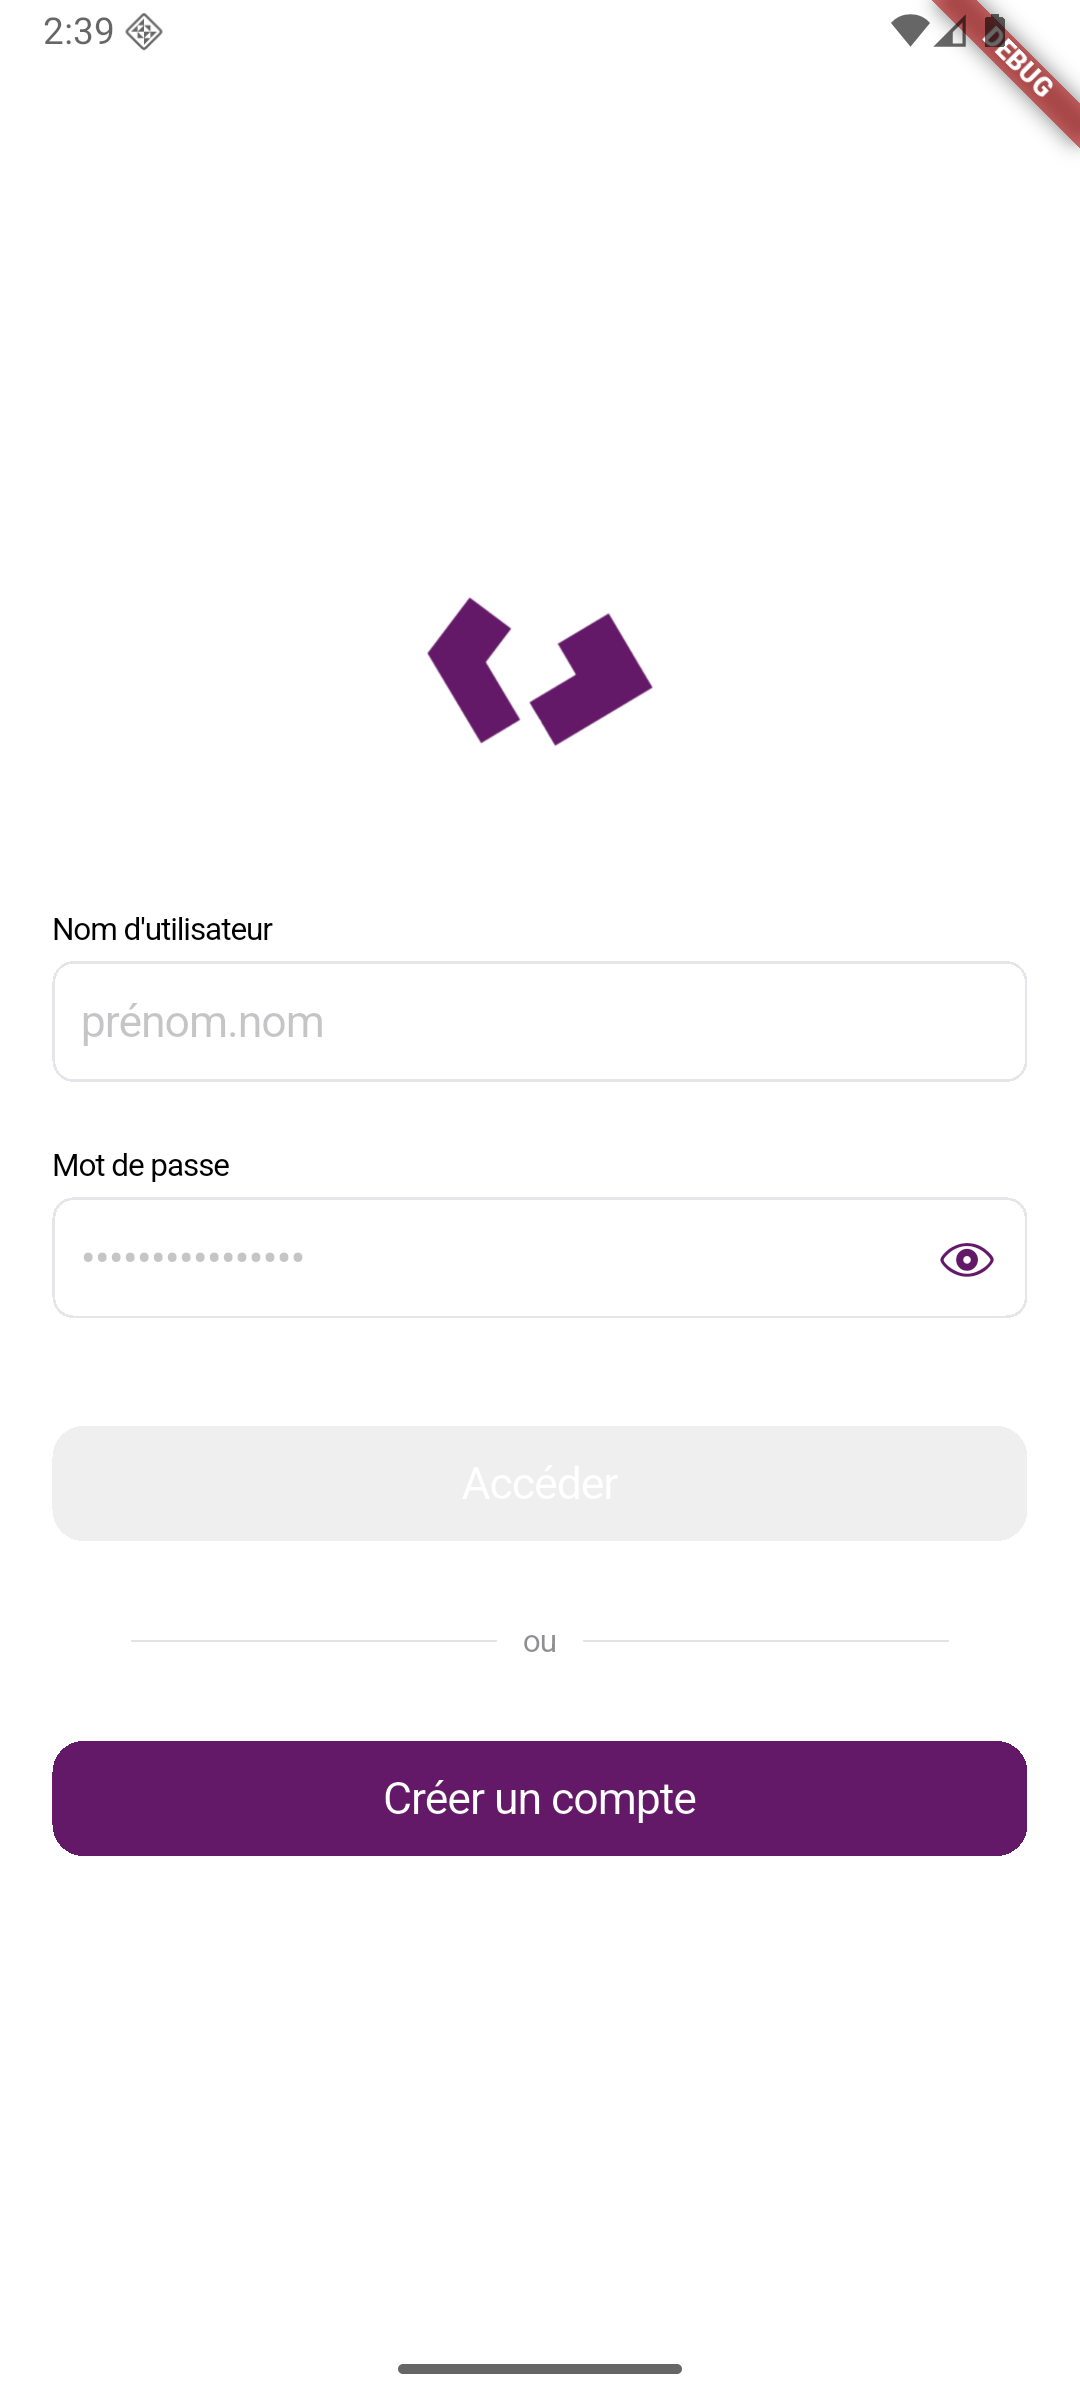
\includegraphics[width=\textwidth]{img/login.png}
			\caption{Page de connexion}
		\end{minipage}
	\end{figure}
	
	\item \textbf{Page d'inscription} : formulaire avec vérification de l’adresse e-mail.
	
	\begin{figure}[H]
		\centering
		\begin{minipage}[t]{0.5\textwidth}
			\centering
			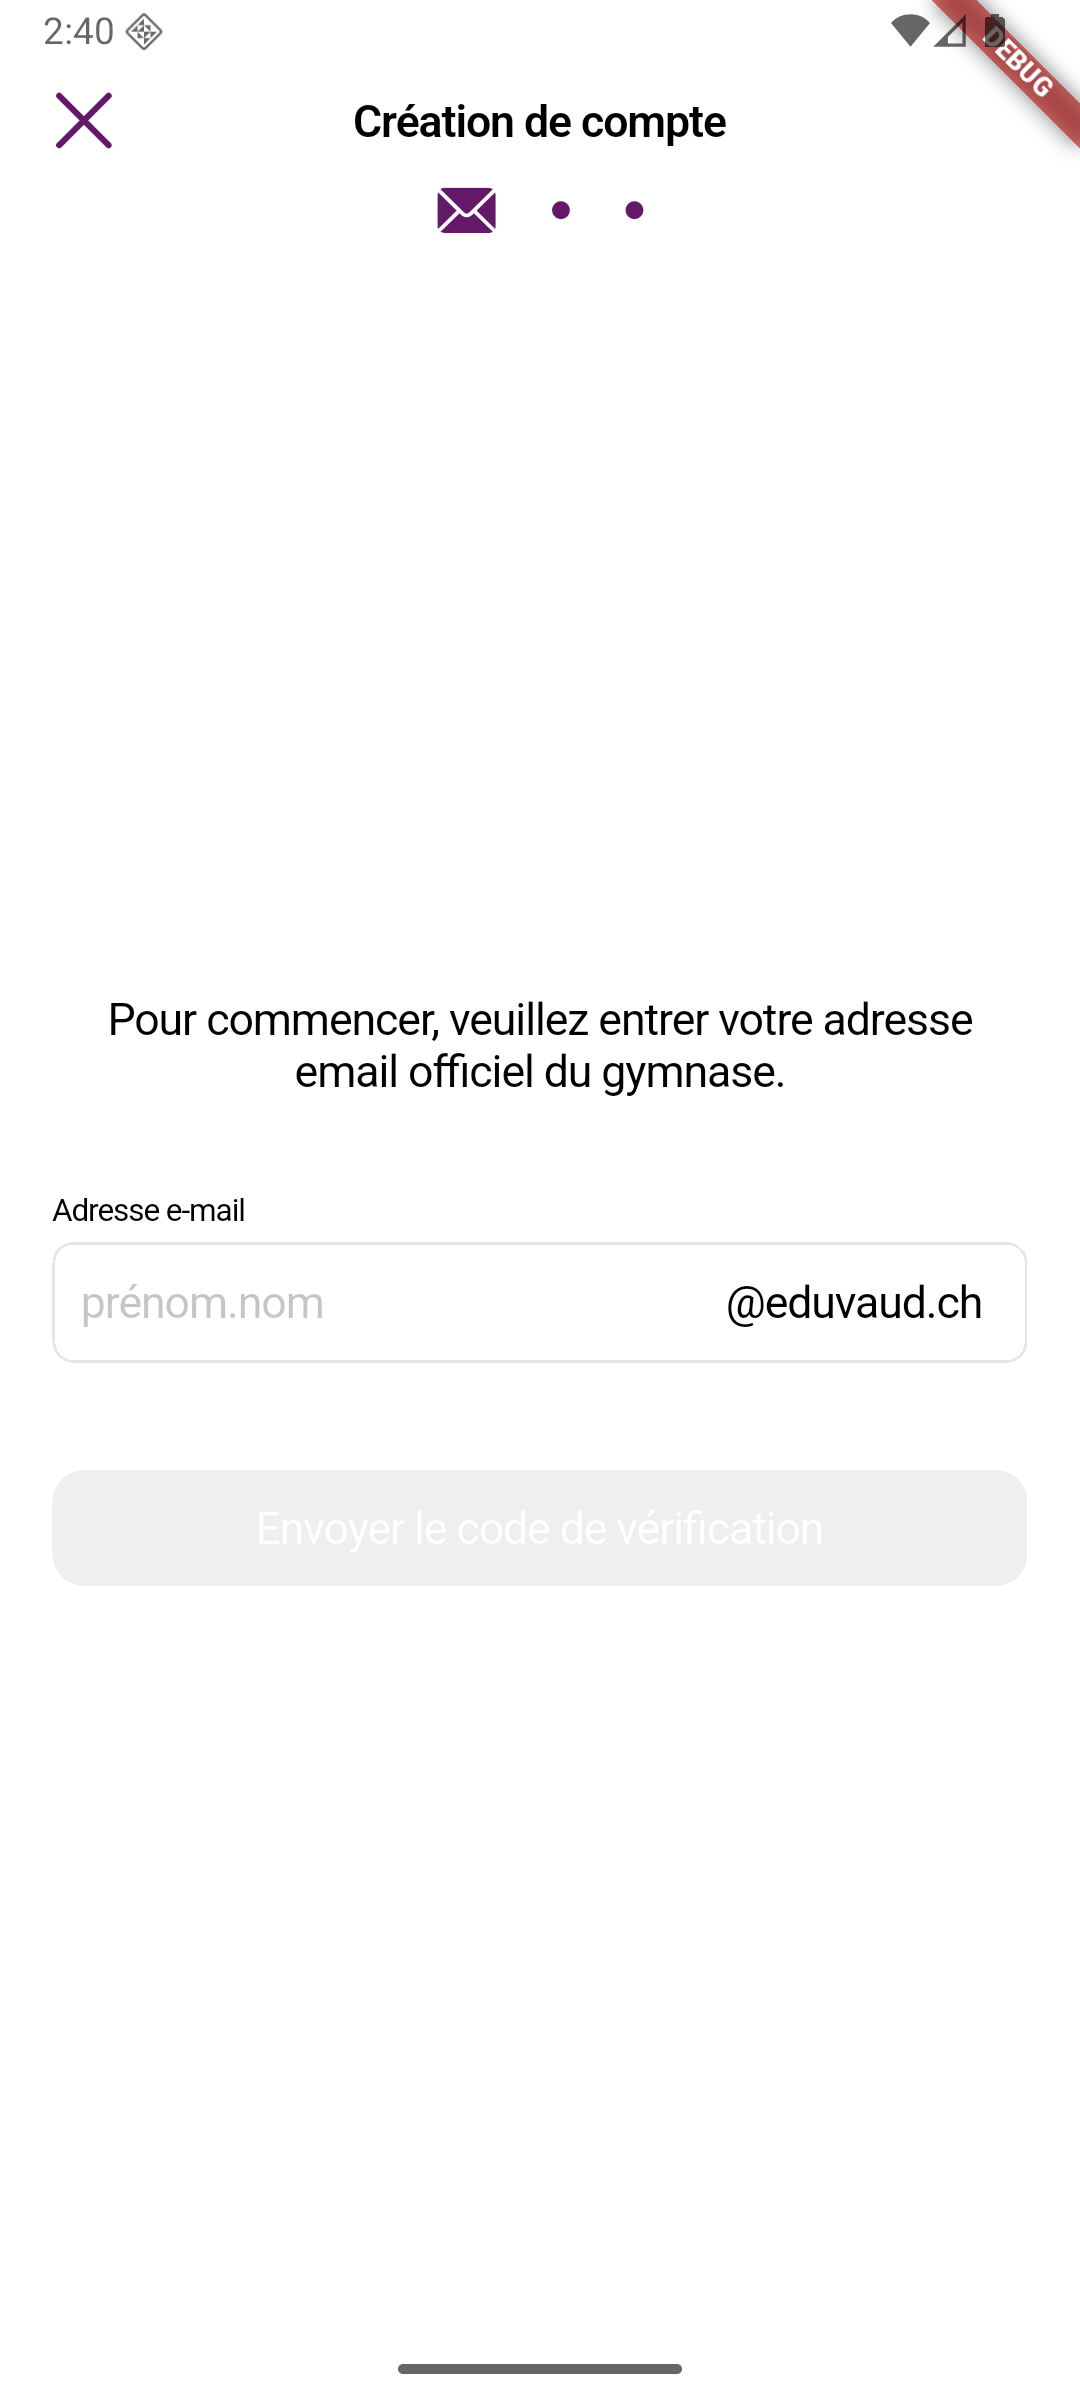
\includegraphics[width=\textwidth]{img/registration_email.png}
			\caption{Page d'inscription}
		\end{minipage}
	\end{figure}
	
	\item \textbf{Liste des conversations} : affichage des contacts et des derniers messages reçus.
	
	\begin{figure}[H]
		\centering
		\begin{minipage}[t]{0.5\textwidth}
			\centering
		%	\includegraphics[width=\textwidth]{img/conversations.png}
			\caption{Liste des conversations}
		\end{minipage}
	\end{figure}
	
	\item \textbf{Fenêtre de discussion} : interface avec les messages envoyés et reçus.
	
	\begin{figure}[H]
		\centering
		\begin{minipage}[t]{0.5\textwidth}
			\centering
		%	\includegraphics[width=\textwidth]{img/chat.png}
			\caption{Fenêtre de discussion}
		\end{minipage}
	\end{figure}
	
	\item \textbf{Profil utilisateur} : aperçu d’un compte avec photo et informations visibles.
	
	\begin{figure}[H]
		\centering
		\begin{minipage}[t]{0.5\textwidth}
			\centering
			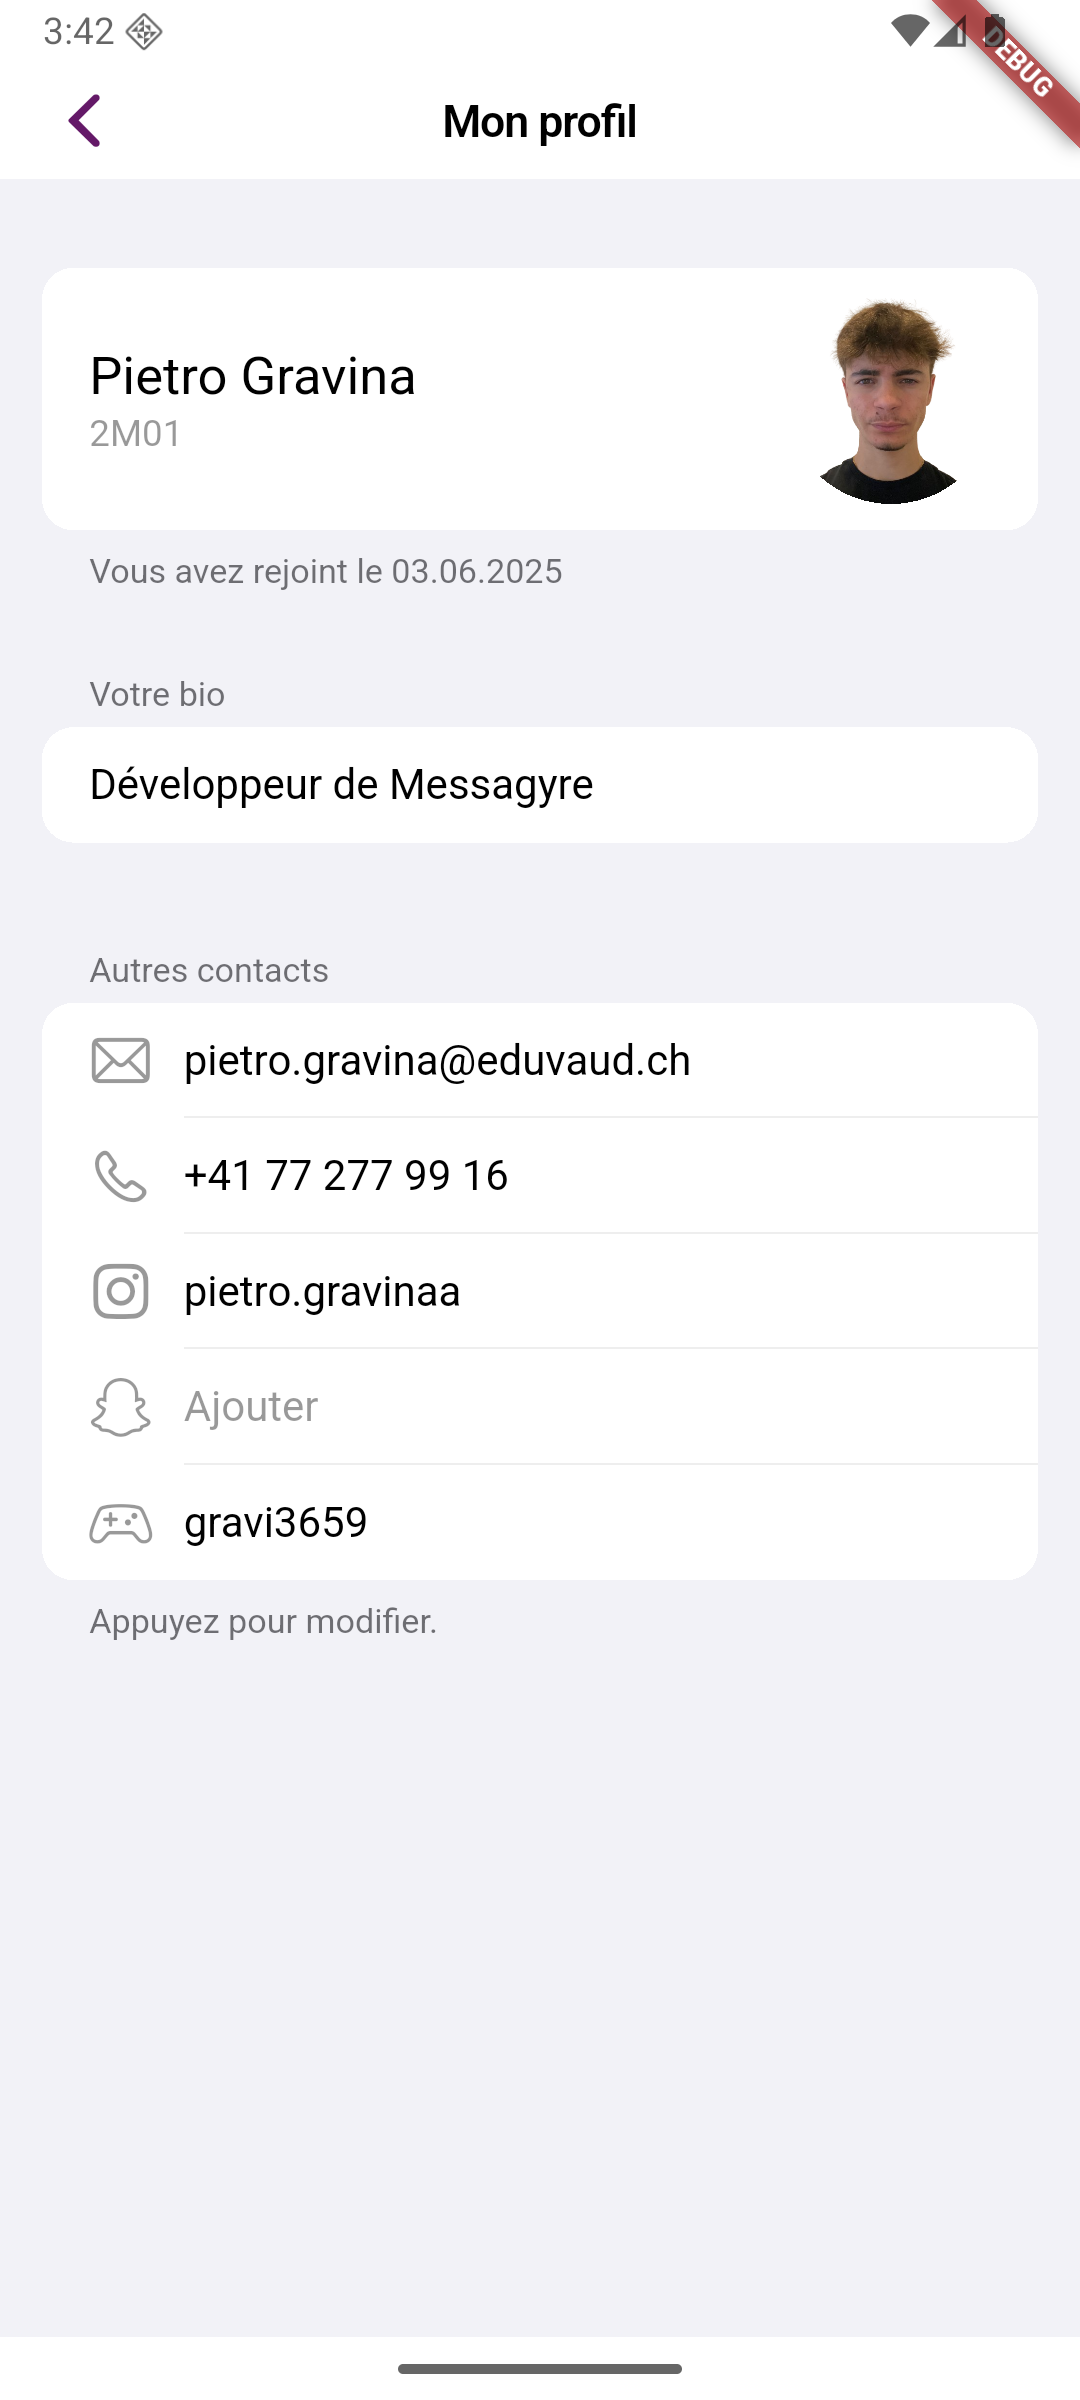
\includegraphics[width=\textwidth]{img/profile.png}
			\caption{Profil utilisateur}
		\end{minipage}
	\end{figure}
	
	\item \textbf{Page des devoirs} : liste des prochains devoirs, ajout d’un nouveau et visualisation des détails.
	
	\begin{figure}[H]
		\centering
		\begin{minipage}[t]{0.32\textwidth}
			\centering
			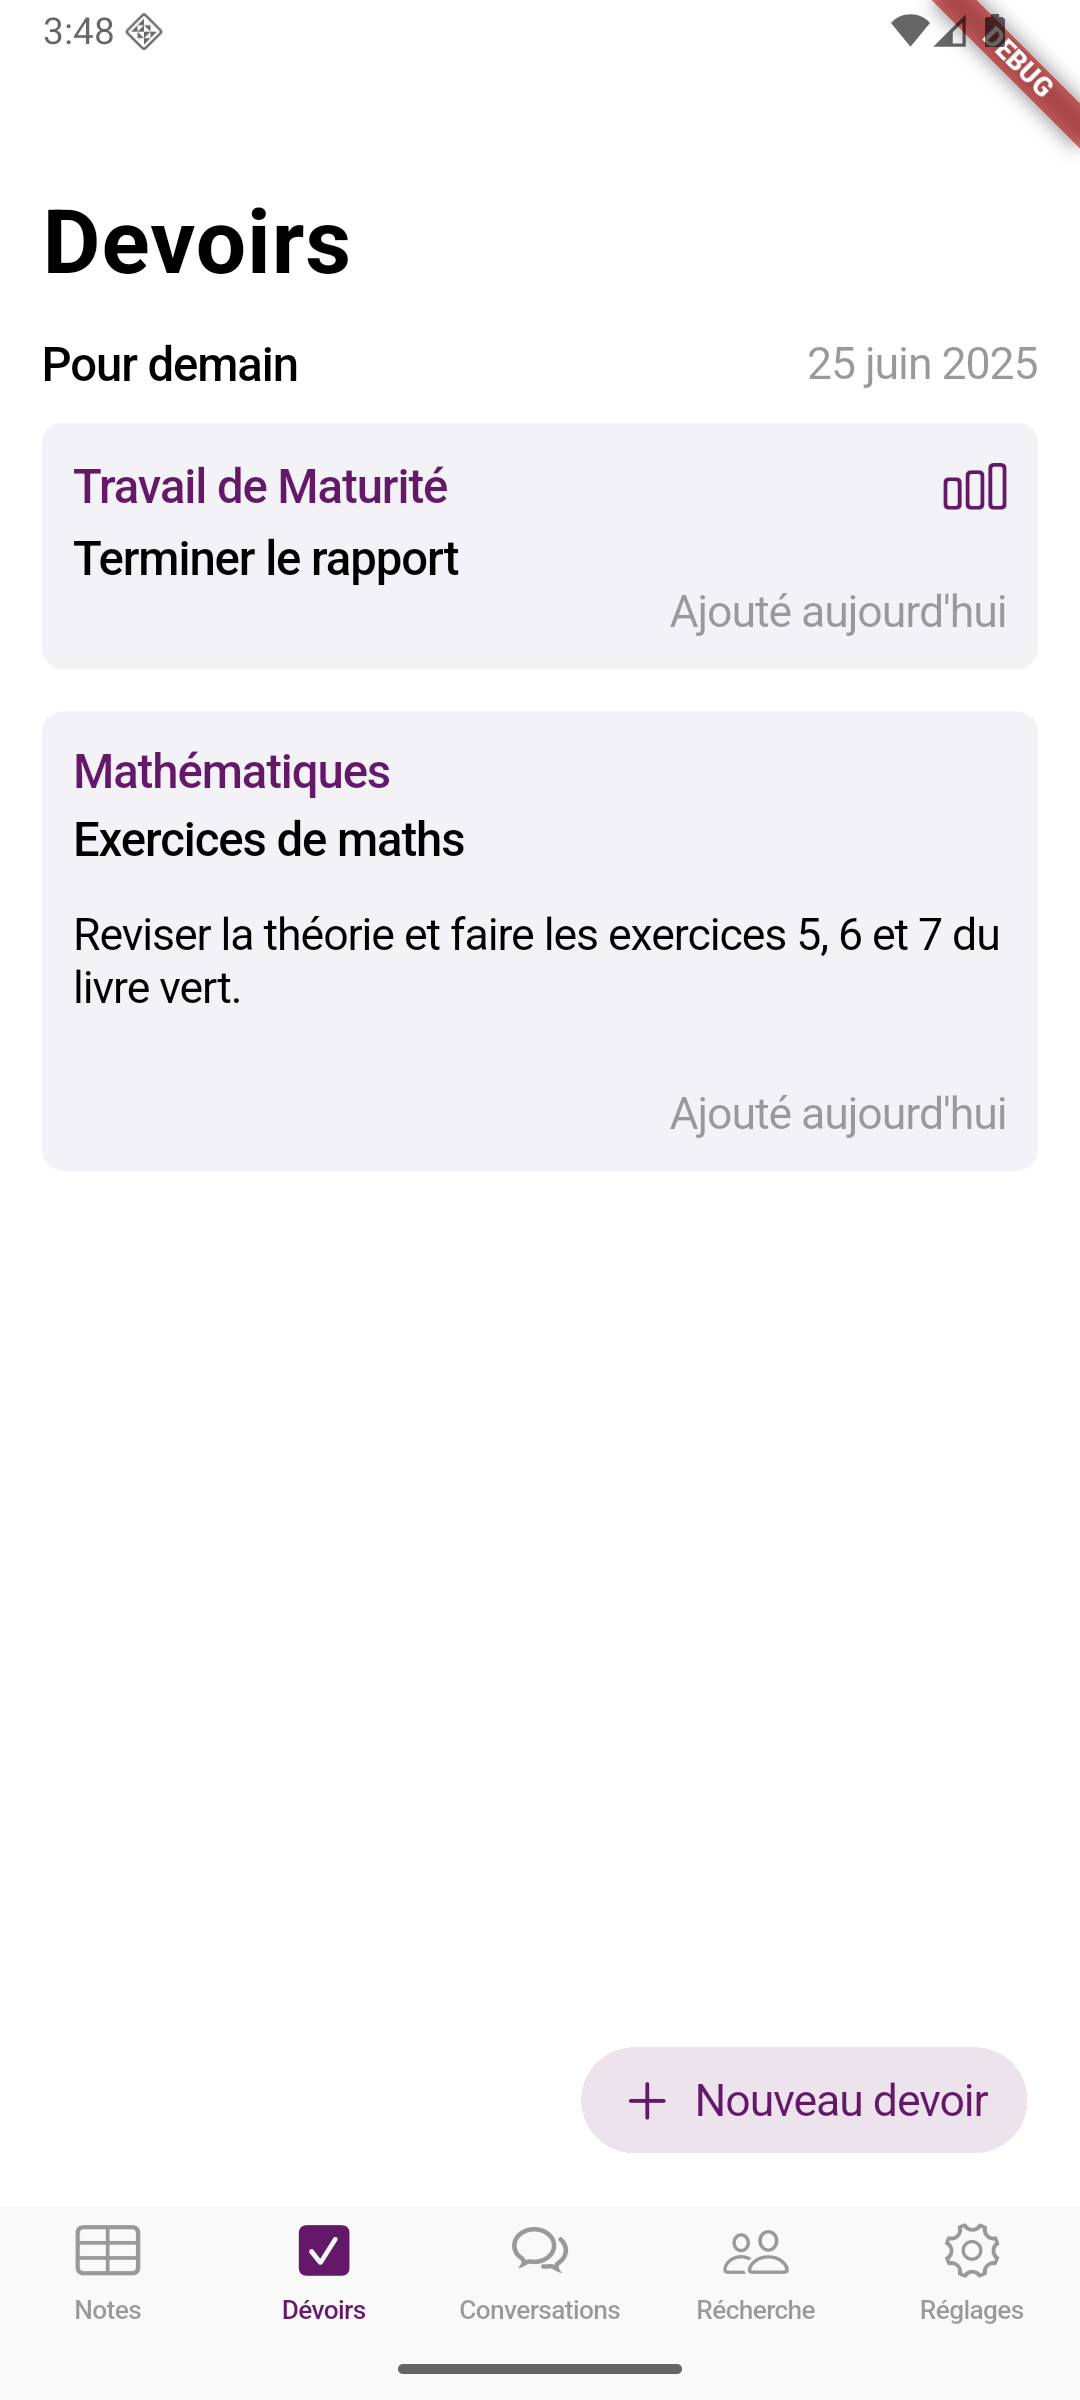
\includegraphics[width=\textwidth]{img/homework.png}
			\caption*{Liste des devoirs}
		\end{minipage}
		\hfill
		\begin{minipage}[t]{0.32\textwidth}
			\centering
			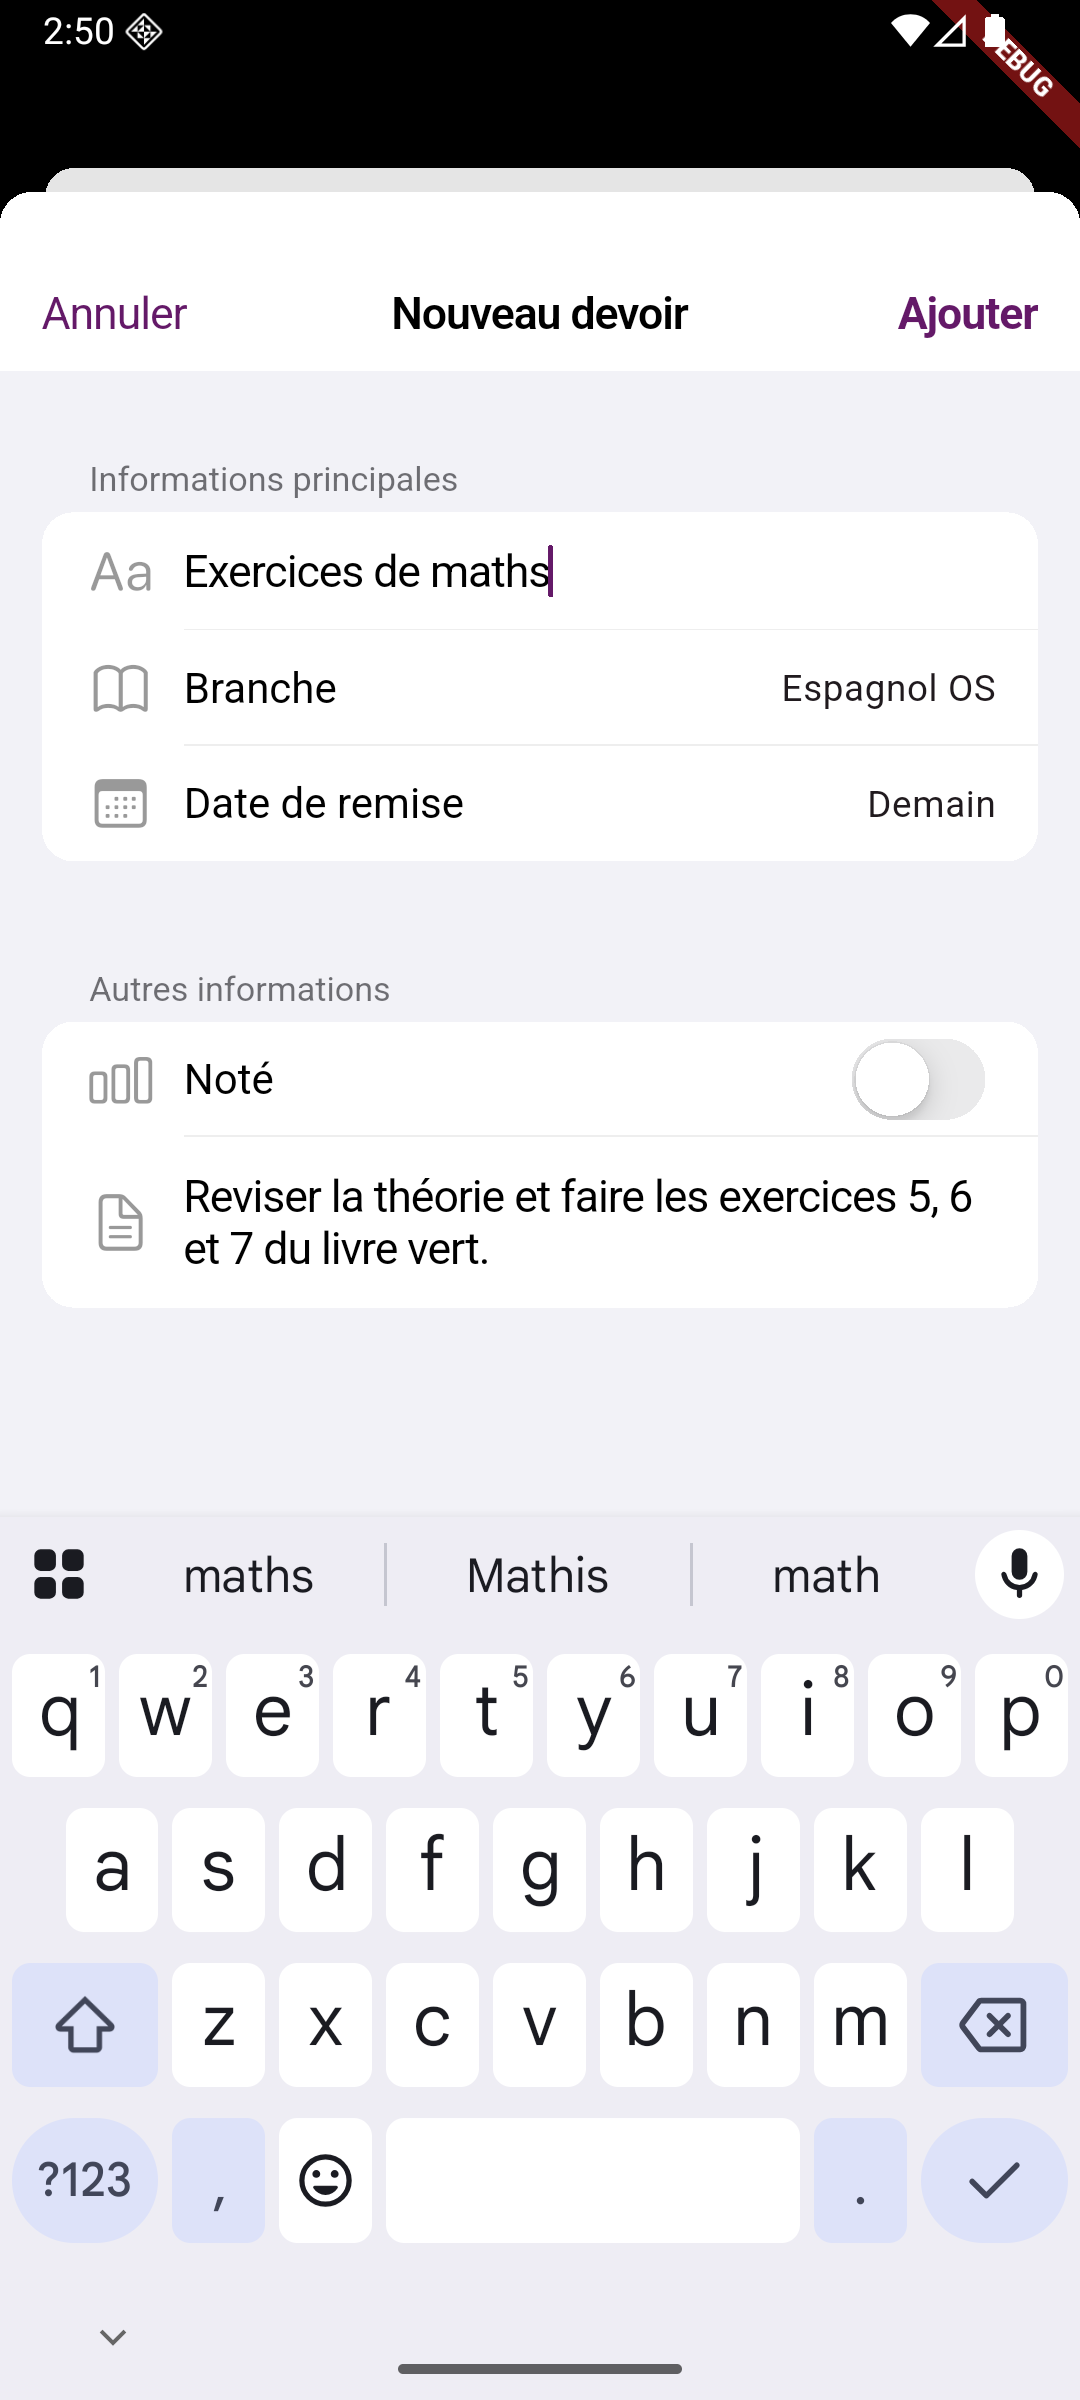
\includegraphics[width=\textwidth]{img/new_homework.png}
			\caption*{Ajout d’un devoir}
		\end{minipage}
		\hfill
		\begin{minipage}[t]{0.32\textwidth}
			\centering
			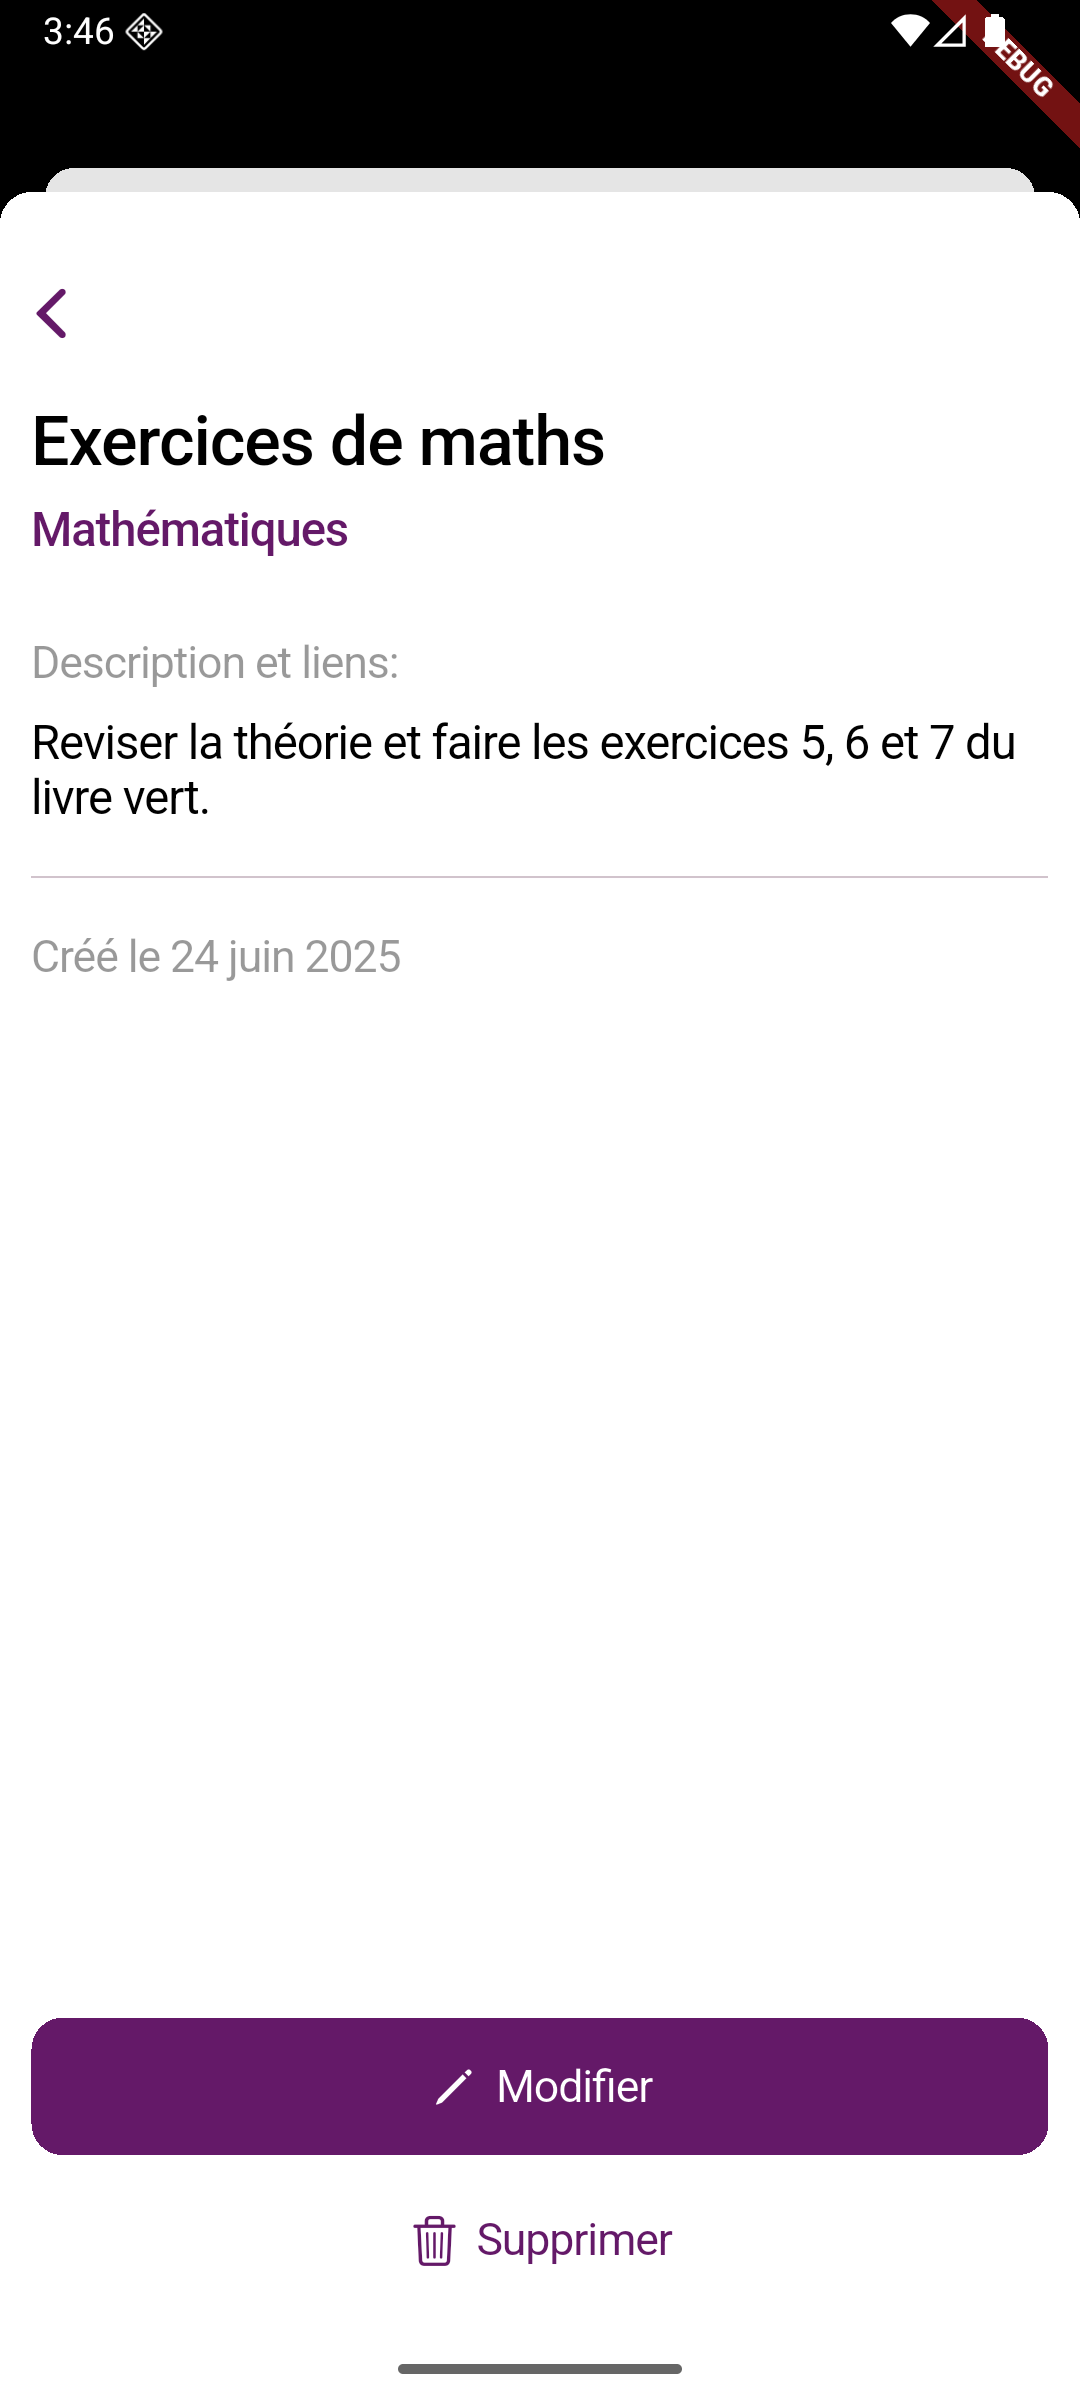
\includegraphics[width=\textwidth]{img/view_homework.png}
			\caption*{Détail d’un devoir}
		\end{minipage}
		\caption{Interface de la page « Devoirs »}
	\end{figure}
	
\end{itemize}



\chapter{Difficultés rencontrées}

\section{Difficultés techniques}

Pendant le développement de Messagyre, j’ai dû faire face à de nombreuses difficultés techniques qui ont mis à l’épreuve mes connaissances et ma capacité d’adaptation.

L’une des premières étapes du projet a été l’utilisation d’Unity comme client. Ce choix initial s’est vite révélé peu adapté au développement d’une application mobile. L’interface utilisateur était plus complexe à construire et les intégrations avec HTTP et WebSocket étaient laborieuses. Chaque élément devait être programmé manuellement : animations, dimensions, positionnement des composants, logique dynamique et visuelle. Tout devait être écrit depuis zéro, sans composants natifs adaptés aux appareils mobiles. Cette gestion artisanale prenait environ 90\% du temps de développement, ralentissant considérablement l’avancement du projet et rendant chaque modification fastidieuse. Le manque d’outils natifs pour les appareils mobiles a nui à l’expérience utilisateur, ce qui m’a poussé à migrer vers Flutter, bien plus adapté à une application moderne et fluide.

Flutter a également posé des difficultés, notamment au début. N’ayant jamais utilisé ce framework auparavant, j’ai eu du mal à comprendre le cycle de vie des widgets et la gestion de l’état. L’intégration de paquets externes pour le chargement d’images, les animations et les notifications m’a demandé de nombreuses tentatives et beaucoup de débogage.

L’un des défis les plus complexes a été la gestion de la communication en temps réel via WebSocket. En plus de devoir comprendre les différences avec HTTP, j’ai appris à gérer des connexions persistantes, des déconnexions inattendues et la synchronisation des messages entre le client et le serveur, tout en garantissant une bonne expérience utilisateur.

La mise en place d’un système d’authentification sécurisé basé sur JWT et RefreshToken a également été une nouveauté pour moi. J’ai étudié des aspects liés à la cryptographie et à la sécurité des données pour assurer la fiabilité des sessions utilisateur. Le volet base de données n’a pas été plus simple : j’ai dû apprendre à configurer et utiliser MySQL, concevoir des tables avec des clés étrangères, optimiser les requêtes et gérer les erreurs de connexion, ce qui a demandé beaucoup de rigueur et de patience.

Le déploiement sur Railway m’a aussi posé des problèmes de compatibilité entre différentes versions de .NET. Adapter le projet à une version stable supportée, sans perdre en performance, a été un défi supplémentaire.

\section{Difficultés organisationnelles}

Outre les aspects techniques, j’ai rencontré des difficultés organisationnelles. Réussir à concilier le développement du projet avec les cours, les devoirs et la vie personnelle n’a pas été simple. J’ai dû apprendre à mieux gérer mon temps, établir des plannings réalistes et éviter la procrastination.

Parfois, la motivation diminuait, surtout dans les moments où les résultats tardaient ou lorsque les problèmes semblaient insurmontables. Mais voir l’application fonctionner concrètement sur le téléphone de mes amis m’a redonné de l’énergie pour continuer.

\section{Comment j’ai surmonté les difficultés}

Pour surmonter ces obstacles techniques et organisationnels, je me suis appuyé principalement sur l’apprentissage autodidacte, avec l’aide précieuse des intelligences artificielles. J’ai consulté la documentation officielle, suivi des tutoriels, lu des discussions sur des forums comme Stack Overflow et GitHub, et expérimenté différentes approches jusqu’à trouver les bonnes solutions.

Les intelligences artificielles se sont révélées être des outils extrêmement efficaces : elles m’ont souvent proposé des solutions optimisées, ce qui m’a fait gagner un temps précieux. Elles m’ont aussi permis d’écrire du code plus propre et de découvrir des bibliothèques ou des paquets que je n’aurais probablement jamais trouvés seul, accélérant ainsi significativement le développement.

J’ai appris à diviser mon travail en objectifs concrets et atteignables, ce qui m’a permis de progresser étape par étape sans me décourager. Parler du projet avec des amis ou des enseignants m’a également aidé à clarifier mes idées et à trouver de nouvelles pistes.

Toutes ces expériences, bien que parfois éprouvantes, m’ont permis de grandir, aussi bien techniquement que dans la gestion de projet et l’autonomie.


\chapter{Bilan personnel}

Ce projet m’a permis de vivre une expérience de développement complète, avec toutes les phases que cela implique : conception, recherche, programmation, tests, déploiement et documentation. Sur le plan technique, j’ai énormément appris. J’ai approfondi mes compétences en C\#, découvert ASP.NET Core, compris en profondeur le fonctionnement des WebSocket et de l’authentification via JWT. J’ai également acquis une grande maîtrise de Flutter et du développement mobile multiplateforme, ainsi que des bases de données MySQL.

Sur le plan personnel, ce travail m’a appris la persévérance, la rigueur et l’autonomie. J’ai dû me former seul sur de nombreuses technologies complexes, souvent sans aide extérieure directe. J’ai aussi pris conscience de l’importance de bien planifier son temps et de savoir demander de l’aide au bon moment. Ce projet m’a donné confiance en ma capacité à mener une idée de bout en bout, même face à des obstacles importants.

Si je devais refaire ce projet, je choisirais dès le départ des outils plus adaptés aux besoins d’une application mobile. J’éviterais Unity, dont la flexibilité est un atout dans le domaine du jeu vidéo, mais un inconvénient majeur dans ce type d’application. J’organiserais aussi mieux mon temps dès le début, avec une feuille de route plus précise et un système de gestion des tâches plus rigoureux.

Quant à l’avenir de Messagyre, je n’exclus pas de continuer à le développer et à l’améliorer. Plusieurs idées restent à concrétiser, comme l’ajout de notifications push, une version web de l’application, l’intégration de messages vocaux ou vidéos, ou encore une meilleure gestion des groupes et des discussions collectives. Le projet pourrait même, un jour, être proposé à d’autres écoles, au-delà du Gymnase de Renens, si son usage s’y prête.

En somme, cette expérience a été à la fois un défi technique et une aventure personnelle très enrichissante, qui m’a beaucoup apporté et dont je suis fier.


\chapter{Conclusion}

Le développement de Messagyre a représenté pour moi un parcours long, exigeant et formateur. De l’idée initiale à la réalisation de l’application, j’ai traversé de nombreuses étapes : changements de technologies, obstacles techniques, réécritures complètes et améliorations successives. Chaque choix, même ceux qui semblaient initialement erronés, a contribué à construire un projet solide et concret.

D’un point de vue technique, j’ai pu expérimenter de manière pratique de nombreuses compétences acquises au fil des années, en consolider de nouvelles et approfondir des technologies complexes comme Flutter, ASP.NET Core, JWT et WebSocket. Mais au-delà des aspects techniques, j’ai acquis une méthode de travail plus organisée et plus consciente, en affrontant des problèmes réels et en apprenant à chercher des solutions efficaces.

Messagyre n’est pas seulement une application de messagerie : c’est le résultat de centaines d’heures de travail, d’essais, d’erreurs et de corrections. C’est aussi la preuve qu’un projet ambitieux peut devenir réalité, même s’il est développé par une seule personne, avec passion et détermination.

Personnellement, je considère ce projet comme l’un des travaux les plus complets et significatifs que j’aie jamais réalisés. Il a une grande valeur, tant du point de vue professionnel — car il démontre mes compétences de développeur — que du point de vue personnel — car il m’a appris à croire en mes idées et à les porter jusqu’au bout avec détermination.

J’espère que Messagyre pourra continuer à évoluer au-delà de ce travail de maturité. Qu’il puisse être utile aux élèves et aux enseignants, et peut-être devenir un véritable outil de communication scolaire, simple, sécurisé et accessible à tous.


\chapter{Sources et bibliographie}

Pour mener à bien le développement de Messagyre, je me suis appuyé sur diverses ressources fiables, disponibles en ligne. Voici les principales :

\section{Documentation officielle}

\begin{itemize}
	\item \textit{Flutter} — \url{https://docs.flutter.dev}
	\item \textit{Flutter API} — \url{https://api.flutter.dev}
	\item \textit{Dart} — \url{https://dart.dev/guides}
	\item \textit{ASP.NET Core} — \url{https://learn.microsoft.com/fr-fr/aspnet/core}
	\item \textit{C\#} (syntaxe et curiosités) — \url{https://learn.microsoft.com/en-us/dotnet/csharp/}
	\item \textit{MySQL} — \url{https://dev.mysql.com/doc/}
	\item \textit{JWT (JSON Web Tokens)} — \url{https://jwt.io/introduction}
	\item \textit{Railway} — \url{https://docs.railway.app}
	\item \textit{pub.dev} — \url{https://pub.dev} : plateforme utilisée pour trouver et installer des paquets et extensions Flutter.
\end{itemize}

\section{Tutoriels, articles et forums}

\begin{itemize}
	\item Stack Overflow — \url{https://stackoverflow.com}
	\item GitHub Discussions — \url{https://github.com}
	\item Flutter Community — \url{https://fluttercommunity.dev}
	\item Railway Community Forum — \url{https://community.railway.app}
	\item TeX Stack Exchange — \url{https://tex.stackexchange.com}
	\item Reddit (r/FlutterDev, r/dotnet, r/webdev) — \url{https://www.reddit.com}
	\item Wikipédia — pages sur \textit{Base64} et \textit{JSON Web Token} pour la compréhension des concepts fondamentaux.
	\item Vidéo YouTube sur CachedNetworkImage (Flutter) — \url{https://www.youtube.com/watch?v=fnHr_rsQwDA&ab_channel=Flutter}
	\item Guide sur CupertinoNavigationBar — \url{https://tillitsdone.com/blogs/cupertino-navigation-bar-guide/}
	\item Installation des drivers Android et utilisation d’ADB — \url{https://androidmtk.com}
	\item Vidéo YouTube sur LargeTitle Cupertino — \url{https://www.youtube.com/watch?v=Uu7s2vigU3A}
	\item Vidéo YouTube sur CupertinoNavigationBar (HeyFlutter) — \url{https://www.youtube.com/watch?v=2M7LidCj_q0&ab_channel=HeyFlutter%E2%80%A4com}
\end{itemize}

\section{Outils d’assistance}

\begin{itemize}
	\item \textbf{ChatGPT (OpenAI)} — pour générer du code, trouver des solutions optimisées et explorer des alternatives techniques.
	\item \textbf{Google Gemini} — pour la recherche de documentation complémentaire et l’exploration d’approches différentes.
	\item \textbf{Claude (Anthropic)} — pour obtenir des résumés techniques et des explications de concepts complexes.
	\item \textbf{Bing AI / Copilot} — pour compléter la recherche de paquets et d’outils adaptés.
\end{itemize}

\section{Outils de développement}

\begin{itemize}
	\item \textbf{Visual Studio 2022} — environnement de développement principal pour ASP.NET Core et le serveur.
	\item \textbf{Visual Studio Code} — utilisé pour éditer des fichiers Dart, JSON, SQL et pour les tests rapides côté client.
	\item \textbf{Android Studio} — utilisé pour installer les SDK Android et tester l’application Flutter via son émulateur intégré.
\end{itemize}

\section{Autres inspirations et connaissances utiles}

\begin{itemize}
	\item Cours de mathématiques sur la cryptographie (Gymnase de Renens) — a contribué à mieux comprendre les principes de sécurité appliqués à l’application (notamment l’utilisation des tokens, des mots de passe hachés et de la confidentialité des échanges).
	\item \textbf{Patternico} — utilisé pour générer les motifs de fond dans les fenêtres de discussion.
	\item \textbf{Pixlr E} — éditeur d’images utilisé pour ajuster et retoucher les visuels de l’application.
	\item \textbf{Google Maps} — utilisé pour dessiner l’icône de l’application à partir de la vue aérienne du bâtiment du gymnase.
	\item \textbf{Remove.bg} — utilisé pour supprimer automatiquement l’arrière-plan de certaines images utilisées dans l’application.
\end{itemize}


\chapter{Annexes}

\section{Code source}

Le code complet du projet est disponible sur GitHub aux adresses suivantes :

\begin{itemize}
	\item \textbf{Client Flutter} : \url{https://github.com/Gravi32/MessagyreClient}
	\item \textbf{Serveur ASP.NET Core} : \url{https://github.com/Gravi32/MessagyreServer}
\end{itemize}

Pour faciliter l’accès, il est possible d’inclure un QR code menant aux dépôts.

\section{Diagrammes}

Pour illustrer la structure et l’architecture du projet, des diagrammes UML ont été réalisés. Le diagramme principal est disponible au lien suivant :

\begin{itemize}
	\item \textbf{Diagramme UML} : \url{https://lucid.app/lucidchart/b8dadd52-61fd-468b-8bd6-a81aa133eb02/edit?viewport_loc=-3637\%2C-1769\%2C9681\%2C4831\%2C0_0&invitationId=inv_fa22bca5-082d-4666-b827-15f4adaa3a38}
\end{itemize}

\section{Icônes de l’application}

Voici les icônes principales utilisées dans Messagyre :

\begin{figure}[H]
	\centering
	\begin{minipage}[t]{0.45\textwidth}
		\centering
		
\includegraphics[width=0.7\textwidth]{img/logo_purple.png}
		\caption{Icône violette (version simplifiée)}
	\end{minipage}
	\hfill
	\begin{minipage}[t]{0.45\textwidth}
		\centering
		
\includegraphics[width=0.7\textwidth]{img/logo_full.png}
		\caption{Icône complète de l’application}
	\end{minipage}
\end{figure}

\chapter{Structure du serveur}

Chaque composant du serveur est expliqué dans les sous-sections à venir, qui présenteront un \textit{"Extrait du code"}, c’est-à-dire une illustration schématique du code du composant. Il est possible de visiter le \href{https://github.com/Gravi32/MessagyreServer.git}{dépôt GitHub} du projet du serveur pour accéder au code complet.
Pour comprendre plus facilement le fonctionnement des différents composants du serveur, un \href{https://lucid.app/lucidchart/b8dadd52-61fd-468b-8bd6-a81aa133eb02/edit?viewport_loc=-3637\%2C-1769\%2C9681\%2C4831\%2C0_0&invitationId=inv_fa22bca5-082d-4666-b827-15f4adaa3a38}{Diagramme UML} est également disponible.

\section{User.cs}

Lorsqu’un serveur reçoit une requête, il est souvent nécessaire de pouvoir reconnaître, distinguer et cataloguer l’expéditeur : cela est représenté par la classe \code{User}, une classe non statique (donc instanciable) contenant toutes les informations utiles concernant l’utilisateur connecté.

\subsection{Extrait du code}
\begin{minted}{csharp}
using System.Net.WebSockets;

namespace MessagyreServer.Classes
{
    public class User
    {
        public Account? Account { get; private set; }
        public WebSocket Socket { get; }
        public bool IsAuthorized { get; private set; }
        public string RegistrationEmailAddress = "";
        public string RegistrationTempEmailAddress = "";
        public int RegistrationVerificationCode;
        public DateTime RegistrationCodeSentAt;
        
        public User(WebSocket Socket)
        {
            this.Socket = Socket;
        }

        public void Receive(Signal SignalToSend)
        {
            Socket.Send(SignalToSend.Pack());
        }

        public void Authenticate(Account? GivenAccount)
        {
            Account = GivenAccount;
            IsAuthorized = GivenAccount != null;
        }
    }
}
\end{minted}

\subsection{Variables principales}
Une instance de la classe \code{User} contient trois informations principales : le compte (\code{Account}) lié à l'utilisateur (si authentifié), le \code{Socket} du client connecté (nécessaire pour pouvoir lui envoyer des messages), et un booléen \code{IsAuthorized} qui indique si l'utilisateur s'est connecté à son compte ou non.

\subsection{Methodes}
Le premier "méthode" de ce script est un \code{Constructor}, il est appelé lorsque la classe est instanciée et stocke le \code{Socket} en mémoire.

Le second est uniquement pour la lisibilité, lorsqu'il est appelé, il envoie le message \code{Signal} au client.

Le dernier (\code{Authenticate()}), est appelé par la classe \code{Authenticator} lorsque l'utilisateur se connecte à son compte.
\\\\

\section{Signal.cs}

Une autre classe non statique qui contient toutes les informations d'une requête/message. Elle est instanciée lorsque le serveur reçoit une requête ou lorsqu'il doit envoyer un message à un client spécifique.

\subsection{Extrait du code}

\begin{minted}{csharp}
using Newtonsoft.Json;

namespace MessagyreServer.Classes
{
	public class Signal
	{
		[JsonIgnore] public User? Sender;

		public SignalType Type;
		public Dictionary<string, string> Data = new();

		public Signal(SignalType Type, User? Sender = null)
		{
			this.Type = Type;
			this.Sender = Sender;
		}

		public string Pack()
		{
			return JsonConvert.SerializeObject(this);
		}
			
		public static Signal? Unpack(string Source, User Sender)
		{
			Signal? Result;

			try { Result = JsonConvert.DeserializeObject<Signal>(Source); }
			catch { return null; }

			if (Result != null) Result.Sender = Sender;

			return Result;
		}
		
	}

	public enum SignalType
	{
		Login, 
		Registration, 
		Logout,
		Message,
		Search
	}
}
\end{minted}

\subsection{Variables principales}
Les informations contenues dans cette classe sont réparties en trois variables :

1.\code{Sender} Indique l'utilisateur à partir duquel le serveur a reçu le message. 
\code{[JsonIgnore]} indique au Serializer de Newtonsoft.Json que la variable ne doit pas être incluse dans le contenu du Json lorsque l'instance de la classe sera stockée en mémoire non volatile. (voir Messages.cs)

2.\code{Type} Indique de quel type de \code{Signal} il s'agit, les options possibles se trouvent dans l’\code{enum} \code{SignalType} en bas du script.

3.\code{Data} Contient un “dictionnaire” (une liste où chaque élément a un nom) avec toutes les données du \code{Signal}, par exemple \code{Username} et \code{Password} dans le cas d'un \code{Signal} de \code{Type} \code{SignalType.Login}.

\subsection{Methodes}
La méthode \code{Pack} “emballe” le \code{Signal}, c'est-à-dire qu'elle convertit les trois variables en un objet \textit{Json} via la méthode \code{SerializeObject} de \code{JsonConvert}, provenant de la bibliothèque \code{Newtonsoft.Json}. Cela est nécessaire pour pouvoir l'envoyer au client, car il n'est pas possible d'envoyer des instances de classes via \textit{WebSocket}, mais uniquement des chaînes de caractères.

\code{Unpack} fait exactement l'inverse, en prenant une chaîne contenant l'objet \textit{Json}, elle la “convertit” en une nouvelle instance de \code{Signal}. Cette action est entourée d'un \code{try catch} car si un client devait envoyer une requête avec des données corrompues, mal formatées ou s'il y avait un problème lors de la transmission, le \textit{Json} ne serait pas valide et le serveur planterait.
\\\\
\section{Account.cs}
Dernière classe non statique qui représente le compte d'un utilisateur.

\subsection{Extrait du code}
\begin{minted}{csharp}
    using Newtonsoft.Json;

namespace MessagyreServer.Classes
{
    public class Account
    {
        public string Username { get; set; }
        public string Password { get; private set; }
        public string EmailAddress { get; set; }
        public DateTime CreationDate { get; }
        public DateTime? LastLogin { get; set; }
        public bool Banned { get; set; }

        public List<Signal> Inbox { get; set; } = new();


        // Constructors 
        public Account(string username, string password, string emailAddress)
        {
            Username = username;
            Password = Hash(password);
            EmailAddress = emailAddress;
            CreationDate = DateTime.UtcNow;
        }

        [JsonConstructor]
        public Account(string username, string password, string emailAddress, DateTime creationDate, DateTime? lastLogin, bool banned)
        {
            Username = username;
            Password = password;
            EmailAddress = emailAddress;
            CreationDate = creationDate;
            LastLogin = lastLogin;
            Banned = banned;
        }



        // Private methods 
        private static string Hash(string Password) => BCrypt.Net.BCrypt.HashPassword(Password);



        // Public methods 
        public bool TryPassword(string Attempt) => BCrypt.Net.BCrypt.Verify(Attempt, Password);

        public static string GetUsernameFromEmail(string Address) => Address.Split('@')[0];

    }
}
\end{minted}

\subsection{Variables}
Cette classe contient toutes les informations d'un compte :

1.\code{Username}: Nom d'utilisateur déduit de l'adresse email de l'utilisateur. (\textit{"prénom.nom"} de l'adresse \textit{"prénom.nom@eduvaud.ch"}) \\
2.\code{Password}: Mot de passe haché (chiffré avec l'algorithme \textit{bcrypt}) utilisant \code{HashPassword} de la bibliothèque \textit{BCrypt.Net}. \\
3.\code{EmailAddress}: Adresse email saisie par l'utilisateur lors de la création de son compte. Sauf exception, le domaine doit obligatoirement être \textit{“@eduvaud.ch”}. \\
4.\code{CreationDate}: Date de création du compte. \\
5.\code{LastLogin}: Date de la dernière connexion à la plateforme.\\
6.\code{Banned}: Valeur booléenne indiquant si l'utilisateur peut accéder à l'application. Si \textit{`true`}, la connexion est refusée. \\

\subsection{Methodes}
Le premier constructeur est appelé par l’\code{Authenticator} lorsque le compte est créé, tandis que le second est appelé par l’\code{AccountsManager} lorsqu'il est chargé en mémoire depuis la base de données. 

La méthode \code{Hash()} est uniquement pour la lisibilité, elle retourne le mot de passe fourni après l'avoir chiffré. \code{TryPassword()} retourne si le mot de passe fourni comme paramètre \code{Attempt} est correct. La méthode \code{GetUsernameFromEmail()} extrait le nom d'utilisateur de l'adresse e-mail.
\\\\

\section{Program.cs (Entry point)}

Point d'entrée du programme, démarrage de l'écoute, gestion et routage des requêtes vers les autres classes.

\subsection{Démarrage du serveur}
\begin{minted}{csharp}
using System.Net.WebSockets;

WebApplicationBuilder Builder = WebApplication.CreateBuilder(args);
WebApplication App = Builder.Build();

[…]

App.UseWebSockets();
App.Use(RequestsHandling);
App.Run();
\end{minted}

Dans le code ci-dessus, l'écoute des requêtes est lancée. Lorsqu'une requête est reçue, la méthode \code{RequestHandling} est appelée et les données de la requête sont transmises en tant qu'arguments de la fonction, comme le \code{Context} et \code{Next}.

\subsection{Gestion des requêtes}
\begin{minted}{csharp}
async Task RequestsHandling(HttpContext Context, Func<Task> Next)
{
    if (Context.WebSockets.IsWebSocketRequest) await OnConnection(Context);
    else await Next();
}
\end{minted}

\code{Context} est une instance de la classe \code{HttpContext} contenant toutes les informations du message \textit{Http} reçu, y compris la propriété \code{IsWebSocketRequest}, qui détermine (intuitivement) si la requête reçue est une requête \textit{WebSocket}. S'il s'agit d'un autre type de requête, alors celle-ci est ignorée et la requête suivante (\code{Next}) est exécutée.

\subsection{Gestion des connexions}

Une fois la requête reçue et déterminé qu’il s’agit d’une requête \textit{WebSocket}, la fonction \code{OnConnection()} suivante est appelée :

\begin{minted}{csharp}
async Task OnConnection(HttpContext HttpRequest)
{
    WebSocket Socket = await HttpRequest.WebSockets.AcceptWebSocketAsync();
    User User = Server.OnConnection(Socket);

    WebSocketReceiveResult? Result = null;
    byte[] Buffer = new byte[1024 * 4];

    do
    {
        try
        {
            Result = await Socket.ReceiveAsync(new ArraySegment<byte>(Buffer), CancellationToken.None);

            string Message = Encoding.UTF8.GetString(Buffer, 0, Result.Count);

            Server.OnSignal(User, Message);
        }
        catch (Exception Ex)
        {
            Log($"Error while receiving: {Ex.Message}");
            break;
        }
    }
    while (!Result.CloseStatus.HasValue && Running);


    Server.OnDisconnection(User);

    if (Socket.State != WebSocketState.Open &&
        Socket.State != WebSocketState.CloseSent &&
        Socket.State != WebSocketState.CloseReceived)
        return;

    await Socket.CloseAsync(WebSocketCloseStatus.NormalClosure, Result?.CloseStatusDescription, CancellationToken.None);
}
\end{minted}

Cette fonction se charge d'accepter les connexions \textit{WebSocket} des clients : Une fois la connexion acceptée et établie, le client est enregistré dans une nouvelle instance de la classe \code{User}, qui est ensuite ajoutée à une liste des utilisateurs connectés.

Ensuite, une boucle est ouverte et se répète tant que la connexion n'est pas fermée, durant laquelle une requête de l'utilisateur connecté est attendue, puis elle est stockée dans le \code{Buffer} et envoyée à la classe \code{Server}.

Pour éviter que d'éventuelles erreurs n'interrompent l'exécution du serveur, l'écoute est entourée d'un \code{try catch}. À la fin de la boucle, c'est-à-dire lorsque la connexion est fermée, la fonction \code{OnDisconnect()} de la classe \code{Server} est appelée pour gérer la déconnexion du client.
\\\\
\section{Server.cs}

Gestion des utilisateurs connectés, du routage des messages vers les autres classes du serveur et des déconnexions.

\begin{minted}{csharp}
namespace MessagyreServer
{
	public static class Server
	{
		public static List<User> ConnectedUsers = new();

		public static User OnConnection(WebSocket Socket)
		{
			User NewUser = new(Socket);
			ConnectedUsers.Add(NewUser);

			return NewUser;
		}

		public static void OnSignal() { ... }

		public static void OnDisconnection(User DisconnectedUser)
		{
			ConnectedUsers.Remove(DisconnectedUser);
		}
	}
}
\end{minted}

Comme mentionné précédemment, la méthode \code{OnConnection()} est appelée par \code{Program} et se charge essentiellement d'instancier la classe \code{User} pour ensuite l'ajouter à la liste des utilisateurs connectés (\code{ConnectedUsers}).

 La méthode \code{OnDisconnection()} est quant à elle appelée lorsque l'utilisateur se déconnecte, le retirant de la liste.

 La méthode principale de cette classe est \code{OnSignal()}:

\begin{minted}{csharp}
public static void OnSignal(User Sender, string JsonSignal)
{
	Signal? ReceivedSignal = Signal.Unpack(JsonSignal, Sender);
	if (ReceivedSignal == null || ReceivedSignal.Sender == null) return;

	// Routing
	switch (ReceivedSignal.Type)
	{
		case SignalType.Login:
			Authenticator.OnLoginSignal(ReceivedSignal);
			break;

		case SignalType.Registration:
			Authenticator.OnRegistrationSignal(ReceivedSignal);
			break;

		case SignalType.Logout:
			Authenticator.OnLogoutSignal(ReceivedSignal);
			break;

		case SignalType.Message:
			Messages.OnMessageSignal(ReceivedSignal);
			break;

		case SignalType.Search:
			AccountsManager.OnSearchSignal(ReceivedSignal);
			break;

	}
}
\end{minted}

Cette méthode reçoit comme arguments une valeur \code{Sender}, c'est-à-dire l'expéditeur de la requête, et un \code{JsonSignal} contenant effectivement le contenu de la requête sous forme de \textit{Json}.

Grâce à ces deux valeurs, une instance de la classe \code{Signal} est créée, puis elle est dirigée vers la classe appropriée, comme la classe \code{Authenticator} pour les demandes de connexion ou la classe \code{Messages} pour les demandes de messagerie.
\\\\
\section{Authenticator.cs}

Il s’occupe de la gestion des accès à la plateforme et de la création des comptes.

\begin{minted}{csharp}
using MailKit.Security;
using MessagyreServer.Classes;
using MimeKit;
using MailKit.Net.Smtp;

namespace MessagyreServer
{
	public class Authenticator
	{
		public static void OnLoginSignal()
		public static void OnRegistrationSignal()
	}
}
\end{minted}

Les types de \code{Signal} gérés ici sont au nombre de deux : 

Ceux de \textit{login} et ceux de \textit{inscription}. Il s'agit de fonctions très longues et une partie du code a été omise ; un lien vers le dépôt \textit{GitHub} est disponible au début du chapitre \textit{“Structure du serveur”}.

\subsection{Login: Accès à un compte existant}

Voici la méthode qui s'occupe de la gestion des \code{SignalType.Login} :

\begin{minted}{csharp}
public static void OnLoginSignal(Signal LoginSignal)
{
    void RespondWith(string Message, string Field = "")
    {
        Signal ResponseSignal = new(SignalType.Login);
        ResponseSignal.Data.Add("Response", Message);
        ResponseSignal.Data.Add("Field", Field);
        LoginSignal.Sender?.Receive(ResponseSignal);
    }

    // Check if all data is there 
    if (LoginSignal.Sender == null) return;
    if (!LoginSignal.Data.TryGetValue("Username", out string? Username)) return;
    if (!LoginSignal.Data.TryGetValue("Password", out string? Password)) return;

    // Check if the account exists 
    if (!AccountsManager.GetAccount(Username, out Account? Account))
    {
        RespondWith("account_not_found", "username");
        return;
    }
    if (Account == null) return;

    // Check the password 
    if (!Account.TryPassword(Password))
    {
        RespondWith("wrong_password", "password");
        return;
    }

    // Check if banned 
    if (Account.Banned)
    {
        RespondWith("banned", "username");
        return;
    }

    // Complete the login
    LoginSignal.Sender.Authenticate(Account);
    RespondWith("success");

    // Sending the inbox content
    foreach (Signal InboxMessage in Account.Inbox) LoginSignal.Sender.Receive(InboxMessage);
}
\end{minted}

Dans cette méthode, une instance de \code{Signal} est fournie en paramètre avec toutes les informations nécessaires à la connexion, le contenu du dictionnaire \code{Content} sera:
\begin{minted}{csharp}
Dictionary<string, string> Content = {
	"Username" : "prénom.nom",
	"Password" : "$2a$12$A/4hYn5TE74CXQm5By0g7Ohx..."
}
\end{minted}

La méthode \code{RespondWith()} est appelée pour envoyer une réponse au client : dans le cas où il y aurait un problème avec les données fournies pour l’accès, la méthode serait appelée avec une chaîne courte en \textit{snake\_case} indiquant le problème, ainsi qu’une autre chaîne représentant la donnée incorrecte. S’il n’y a aucun problème, la méthode est appelée avec la chaîne \code{”success”}.

La première chose vérifiée à la réception du signal est la présence des données : si l’expéditeur ou l’une des deux données est nulle, la requête est annulée.

Ensuite, on vérifie s’il existe effectivement un compte correspondant au nom d’utilisateur donné, si le mot de passe correspond, et si la personne n’est pas bannie de la plateforme.

Si ces contrôles sont concluants, la procédure de connexion à la plateforme est finalisée, donnant accès au client, et tous les éventuels messages envoyés à l’utilisateur pendant son absence sont transmis.

\subsection{Registration: Creation d'un nouveau compte}

En ce qui concerne les signaux de \textit{inscription}, la gestion de ces requêtes est nettement plus complexe : lorsque le client envoie son adresse e-mail au serveur pour créer un nouveau compte, il est nécessaire de vérifier qu’il s’agit bien du véritable propriétaire de l’adresse, afin d’éviter la création de comptes au nom d’une autre personne. Ce contrôle supplémentaire rend le processus d’authentification beaucoup plus long et complexe.

\begin{minted}{csharp}
public static void OnRegistrationSignal(Signal RegistrationSignal)
{
    var Sender = RegistrationSignal.Sender;
    var Data = RegistrationSignal.Data;

    if (Sender == null || Data == null) return;


    void RespondWith(string Message, string Field = "") { ...}

    void SendVerificationEmail(string TargetAddress, int Code)
    {
        // Configurations
        string SmtpServer = "smtp.gmail.com";
        int SmtpPort = 587;
        string SenderEmail = "messagyre@gmail.com";
        string SenderPassword = "ywgm otfr qgam pbmz";
        string EmailContentPath = Path.Combine(AppContext.BaseDirectory, "Assets", "VerificationCodeEmail.html");

        // Creating the email
        var Email = new MimeMessage();
        Email.From.Add(new MailboxAddress("Messagyre", SenderEmail));
        Email.To.Add(new MailboxAddress("", TargetAddress));
        Email.Subject = "Verification Code";

        string EmailContent = string.Empty;
        if (File.Exists(EmailContentPath)) EmailContent = File.ReadAllText(EmailContentPath).Replace("{{CODE}}", Code.ToString());

        Email.Body = new TextPart("html") { Text = EmailContent };


        // Connecting to the SMTP server and sending the email
        using var TempClient = new SmtpClient();

        TempClient.Connect(SmtpServer, SmtpPort, SecureSocketOptions.StartTls);
        TempClient.Authenticate(SenderEmail, SenderPassword);
        TempClient.Send(Email);
        TempClient.Disconnect(true);

    }



    /* User sent e-mail address */
    if (Data.TryGetValue("email_address", out string? Address))
    {
        // Checking if the given address is valid 
        if (!Address.Contains('@') || !Address.Contains('.'))
        {
            RespondWith("wrong_format", "email_address");
            return;
        }
        if (!Address.EndsWith("@eduvaud.ch"))
        {
            RespondWith("wrong_domain", "email_address");
            return;
        }
        if (AccountsManager.GetAccount(Account.GetUsernameFromEmail(Address), out var _))
        {
            RespondWith("already_exists", "email_address");
        }
        if ((DateTime.UtcNow - Sender.RegistrationCodeSentAt).TotalMinutes < 2)
        {
            RespondWith("wait", "email_address");
        }

        // Creating the verification code and storing it for the next step
        int VerificationCode = new Random().Next(100000, 1000000);
        Sender.RegistrationVerificationCode = VerificationCode;
        Sender.RegistrationTempEmailAddress = Address;
        Sender.RegistrationCodeSentAt = DateTime.UtcNow;

        // Proceeding
        RespondWith("success", "email_address");
        SendVerificationEmail(Address, VerificationCode);
        Log($"VerificationCode sent to {Address}: {VerificationCode}");
    }

    /* User sent verification code */
    else if (Data.TryGetValue("verification_code", out string? Code))
    {
        if (Code.Length != 6)
        {
            RespondWith("wrong_length", "verification_code");
            return;
        }
        if (Code != Sender.RegistrationVerificationCode.ToString())
        {
            RespondWith("wrong", "verification_code");
            return;
        }

        Sender.RegistrationEmailAddress = Sender.RegistrationTempEmailAddress;

        RespondWith("success", "verification_code");
    }

    /* User sent password */
    else if (Data.TryGetValue("password", out string? Password))
    {
        if (Password.Length < 8)
        {
            RespondWith("too_short", "password");
            return;
        }

        string EmailAddress = Sender.RegistrationEmailAddress;
        string Username = Account.GetUsernameFromEmail(EmailAddress);

        Account NewAccount = new(Username, Password, EmailAddress);
        AccountsManager.AddAccount(NewAccount);
        Sender.Authenticate(NewAccount);

        RespondWith("success", "password");

        Log($"{Username} connected", true);
    }
}
\end{minted}

Cette fonction est divisée en trois sections principales :
\\

1. La gestion de l’adresse e-mail.

\begin{itemize}
    \item On vérifie d'abord si la valeur est effectivement fournie et n'est pas nulle ;
    \item L’adresse doit contenir au moins un point (\textit{“.”}) et une arobase (\textit{“@”}) ;
    \item Le domaine de l’adresse doit être “@eduvaud.ch” ;
    \item Il ne doit pas déjà exister un compte associé à cette adresse ;
    \item L’utilisateur ne doit pas avoir déjà tenté de créer un compte moins de deux minutes avant la tentative actuelle.
\end{itemize}

Si toutes les conditions sont remplies, un e-mail est envoyé à l’adresse donnée, depuis l’adresse \textit{"messagyre@gmail.com"} créée exclusivement pour le développement de cette application, à laquelle le programme accède automatiquement grâce aux identifiants écrits dans le fichier (\code{SmtpPort}, \code{SenderEmail}, \code{SenderPassword}). Le contenu de l’e-mail est chargé depuis le fichier \textit{HTML} \code{VerificationCodeEmail.html}, situé dans le dossier \textit{Assets} du répertoire du serveur. Pour envoyer l’e-mail, un client temporaire doit être créé pour se connecter au serveur \textit{SMTP} (Simple Mail Transfer Protocol, serveur de gestion des e-mails).
\\

2. La gestion du code de vérification.

\begin{itemize}
    \item Le code ne doit pas être plus court ou plus long que six chiffres ;
    \item Le code doit correspondre à celui envoyé.
\end{itemize}

Si le code correspond, alors l’adresse est vérifiée et l’on peut passer à la dernière étape de l’inscription.
\\

3. La création du mot de passe.

\begin{itemize}
    \item Il doit avoir une longueur minimale de 8 caractères.
\end{itemize}

Si le mot de passe respecte cette condition, le compte est créé avec succès, et l’utilisateur accède à l’application.
\\\\

\section{AccountsManager.cs}
Elle s’occupe de la gestion des comptes, de leur sauvegarde en mémoire, mais aussi de fournir les résultats lorsqu’un utilisateur recherche un autre compte.

\subsection{Extrait du code}
\begin{minted}{csharp}
using MySql.Data.MySqlClient;
using MessagyreServer.Classes;
using Newtonsoft.Json;
using System.Data;

namespace MessagyreServer
{
	public static class AccountsManager
	{
		private static readonly string ConnectionString ="Server=metro.proxy.rlwy.net;Port=17551;Database=railway;User=root;Password=uGZBAjgfYSXFTcfJDWySgEVBxjScuDwB;\r\n";
		
		public static bool GetAccount(string Username, out Account? Result) {...}
		
		public static void AddAccount(Account NewAccount) {...}
		
		public static void DeleteAccount(string Username) {...}

		public static List<string> SearchAccount(string Query) {...}
		
		public static void OnSearchSignal(Signal SearchSignal)
		{
			if (SearchSignal.Sender == null) return;
			if (!SearchSignal.Data.TryGetValue("Query", out string? Query)) return;
			
			Signal ResponseSignal = new(SignalType.Search);
			ResponseSignal.Data.Add("Result", JsonConvert.SerializeObject(SearchAccount(Query)));
			SearchSignal.Sender?.Receive(ResponseSignal);
		}
	}
}
\end{minted}

\subsection{Variables}
In questo codice l'unica variabile globale presente è \code{ConnectionString}. Si tratta di una stringa di testo contenente tutte le informazioni necessarie per la connessione al server SQL. In questo caso la \code{ConnectionString} permette al programma di connettersi al database \textit{MySQL} in esecuzione sempre sulla piattaforma \textit{Railway.app}. Le informazioni contenute nella stringa sono\\ 
1.\code{Server}: indica l'indirizzo del database SQL. Può essere un \textit{IP}, un nome o \textit{"localhost"} se è in esecuzione in locale. Per evitare spese inutili, per testare le funzionalità del server durante lo sviluppo, ho usato quest'ultima opzione.\\
2.\code{Port}: indica la porta sulla quale il server ascolta le richieste SQL.\\ 
3.\code{Database}: è il nome del database al quale il server si deve collegare.\\
4.\code{User} e \code{Password}: le credenziali necessarie per accedere al database e eventualmente modificarne proprietà e contenuti.

\subsection{Obtention d'un compte}

Questo metodo qui sotto viene chiamato principalmente dall \code{Authenticator} per ottenere un account oppure per verificarne l'esistenza. Perché funzioni, è necessario fornire un parametro \code{Username}, cioè il nome utente dell'account in questione; \code{Result} non è un parametro, come dimostrato dalla \textit{keyword} \code{out}, bensi un modificatore di parametro, l'ho utilizzato in questo caso per poter restituire due valori da un singolo metodo, cosa non possibile cambiandone solo il tipo. Infatti questo metodo restituisce un valore booleano indicante l'esistenza dell'account ricercato, mentre \code{Result} ottiene come valore il "risultato" dell'operazione, ovvero l'account trovato.kla

\begin{minted}{csharp}
public static bool GetAccount(string Username, out Account? Result)
{
	string Query = "SELECT 
		Username, 
		Password, 
		EmailAddress, 
		CreationDate, 
		LastLogin, 
		Banned 
		FROM Account WHERE Username = @Username";
	Result = null;
	
	// Connecting to the SQL server
	MySqlConnection Connection = new(ConnectionString);
	Connection.Open();
	
	// Creating the command
	MySqlCommand Command = new(Query, Connection);
	Command.Parameters.AddWithValue("@Username", Username);
	
	// Sending the command and reading the response
	var Reader = Command.ExecuteReader();
	if (!Reader.Read()) return false; // No result
	
	Result = new Account(
	Reader.GetString("Username"),
	Reader.GetString("Password"),
	Reader.GetString("EmailAddress"),
	Reader.GetDateTime("CreationDate"),
	Reader.IsDBNull("LastLogin") ? null : Reader.GetDateTime("LastLogin"),
	Reader.GetBoolean("Banned")
	);
	
	return true;
}
\end{minted}
Le azioni eseguite in questo metodo sono tipiche di una richiesta SQL con risultato:
\begin{itemize}
	\item 1. Creazione della \code{Query}, cioè la richiesta da inviare al database;
	\item 2. Connessione al database;
	\item 3. Creazione di un istanza di \code{Command}, necessaria per la gestione della comunicazione col server SQL;
	\item 4. Invio del comando e l'attesa della risposta, entrambi gestiti da \code{Command.ExecuteReader()}.
	\item 5. Lettura della risposta del server, \code{Reader.Read()} restituisce \textit{true} se il server ha risposto con almeno una riga di testo, \textit{false} in caso contrario.
	\item 6. Instanziamento della classe \code{Account}, contenente le informazioni ottenute.
	\item 7. Restituzione di un valore \code{true}, indicante il successo dell'operazione.
\end{itemize}
Il comportamento del codice qui sopra è anche spiegato in inglese nei commenti (\textit{"Connessione al server SQL"}, \textit{"Creazione del comando"}, \textit{"Invio del comando e attesa della risposta"}).

\subsection{Creation d'un compte}
Questo metodo invece viene chiamato quando è necessario creare un nuovo account. L'\code{Authenticator} ne fa uso quando un utente completa l'ultima tappa della \textit{registration}. Per l'esecuzione di questo metodo è richiesto un solo parametro, un'istanza della classe \code{Account} contenente tutte le informazioni dell'account da aggiungere al database.

\begin{minted}{csharp}
public static void AddAccount(Account NewAccount)
{
	if (GetAccount(NewAccount.Username, out var _)) return;
	
	string Query = "INSERT INTO Account (Username, Password, EmailAddress, CreationDate, LastLogin, Banned) VALUES (@Username, @Password, @EmailAddress, @CreationDate, @LastLogin, @Banned)";
	
	MySqlConnection Connection = new(ConnectionString);
	Connection.Open();
	MySqlCommand Command = new(Query, Connection);
	
	Command.Parameters.AddWithValue("@Username", NewAccount.Username);
	Command.Parameters.AddWithValue("@Password", NewAccount.Password);
	Command.Parameters.AddWithValue("@EmailAddress", NewAccount.EmailAddress);
	Command.Parameters.AddWithValue("@CreationDate", NewAccount.CreationDate);
	Command.Parameters.AddWithValue("@LastLogin", (object?) NewAccount.LastLogin ?? DBNull.Value);
	Command.Parameters.AddWithValue("@Banned", NewAccount.Banned);
	Command.ExecuteNonQuery();
}
\end{minted}

La prima cosa controllata all'esecuzione del metodo, è l'esistenza di un altro account con lo stesso nome utente nel database. Questo controllo viene effettuato col fine di evitare conflitti con altri account omonimi. Il resto delle azioni sono simili al metodo precedente, con la differenza che questo non invia una richiesta con risultato, bensi un semplice comando. Invece di attendere una risposta dal server, come visto precedentemente con \code{Command.ExecuteReader()}, il metodo chiamato è \code{Command.ExecuteNonQuery()}, che invia unicamente il comando.

\subsection{Suppression d'un compte}

Metodo chiamato per eliminare un account. Anche in questo caso è richiesto un solo parametro, una stringa \code{Username} rappresentante il nome utente assegnato all'account da eliminare. 

\begin{minted}{csharp}
public static void DeleteAccount(string Username)
{
	string Query = "DELETE FROM Account WHERE Username = @Username";
	
	MySqlConnection Connection = new(ConnectionString);
	Connection.Open();
	MySqlCommand Command = new(Query, Connection);
	
	Command.Parameters.AddWithValue("@Username", Username);
	Command.ExecuteNonQuery();
}
\end{minted}

La struttura è la medesima del metodo precedente, trattandosi di un comando senza risposta.

\subsection{Recherche d'un compte}

Metodo chiamato quando un utente, dalla barra di ricerca nella pagina \textit{"Conversations"} dell'applicazione Messagyre, inserisce almeno due caratteri per cercare un altro utente.
Questo metodo richiede come parametro la stringa immessa dall'utente nella sua barra di ricerca, da notare che questa stringa potrebbe non essere il nome utente completo, bensi una parte di almeno due caratteri di lunghezza.

\begin{minted}{csharp}
public static List<string> SearchAccount(string Query)
{
	string SqlQuery = "SELECT Username FROM Account WHERE Username LIKE @Query";
	
	List<string> Results = new();
	
	MySqlConnection Connection = new(ConnectionString);
	Connection.Open();
	
	MySqlCommand Cmd = new(SqlQuery, Connection);
	Cmd.Parameters.AddWithValue("@Query", "%" + Query + "%");
	
	var Reader = Cmd.ExecuteReader();
	
	while (Reader.Read()) Results.Add(Reader.GetString("Username"));
	
	return Results;
}
\end{minted}

La struttura è quella di una richiesta con risposta, con la differenza che in questo caso ci possono essere molteplici risultati. Verrà infatti restituita una lista \code{Results} con tutti i valori inviati dal database e letti da \code{Reader.Read()}, che legge la risposta riga per riga.

\section{Messages.cs}

Quando un utente invia un messaggio a un altro utente, questo messaggio viene inviato al server, che lo gestisce e lo reindirizza all'utente destinatario.

\subsection{Extrait du code}

\begin{minted}{csharp}
using MessagyreServer.Classes;

public class Messages
{
	public static void OnMessageSignal(Signal MessageSignal) {...}
	
	public static void SendMessage(string SenderUsername, string RecipientUsername, string Content) {...}
}
\end{minted}

\subsection{Reception d'un message}

Quando il server riceve un segnale con il valore della variabile \code{Type} pari a \code{SignalType.Message}, la classe \code{Server} chiama il metodo \code{OnMessageSignal()}, fornendo come parametro il segnale ricevuto.

\begin{minted}{csharp}
public static void OnMessageSignal(Signal MessageSignal)
{
	// Checking if the sender is logged in
	if (!MessageSignal.Sender!.IsAuthorized) return;
	
	// Getting the data
	if (!MessageSignal.Data.TryGetValue("RecipientUsername", out string? RecipientUsername)) return;
	if (!MessageSignal.Data.TryGetValue("Content", out string? Content)) return;
	string SenderUsername = MessageSignal.Sender.Account!.Username;
	
	// Sending
	SendMessage(SenderUsername, RecipientUsername, Content);
}
\end{minted}

Quando viene chiamato il metodo, viene innanzitutto controllato se l'utente dal quale client il server ha ricevuto il segnale sia \textit{autentificato}, cioè abbia effettuato l'accesso alla piattaforma: in caso contrario, l'utente non dovrebbe essere in grado di inviare messaggi perché l'applicazione non dovrebbe permetterlo, quindi il segnale viene ignorato.
In seguito vengono ottenuti i dati dal segnale: l'\code{Username} del destinatario e il contenuto (\code{Content}) del messaggio. 
Infine viene inviato il messaggio, chiamando il metodo \code{SendMessage}, trattato nella seguente sezione.

\subsection{Envoi d'un message}

Come visto precedentemente, per l'invio di un messaggio a partire dal server, viene chiamato il metodo \code{SendMessage}, che si occupa di recapitare il messaggio all'utente, che questo sia attualmente connesso alla piattaforma oppure no. I parametri richiesti sono il nome utente del mittente (\code{SenderUsername}), quello del destinatario (\code{RecipientUsername}) e il contenuto del messaggio (\code{Content}).

\begin{minted}{csharp}
public static void SendMessage(string SenderUsername, string RecipientUsername, string Content)
{
	// Getting the recipient account
	if (!AccountsManager.GetAccount(RecipientUsername, out Account? RecipientAccount)) return;
	
	// Checking if the recipient is online
	User? Recipient = null;
	foreach (User ConnectedUser in Server.ConnectedUsers)
	{
		if (ConnectedUser.Account?.Username == RecipientUsername) Recipient = ConnectedUser;
	}
	
	// Creating the message signal
	Signal NewMessageSignal = new(SignalType.Message);
	NewMessageSignal.Data.Add("SenderUsername", SenderUsername);
	NewMessageSignal.Data.Add("Content", Content);
	NewMessageSignal.Data.Add("SentAt", DateTime.UtcNow.ToString("o"));
	
	// Sending to the online user or to their inbox
	if (Recipient != null)
	{
		Recipient.Receive(NewMessageSignal);
	}
	else
	{
		RecipientAccount!.Inbox.Add(NewMessageSignal);
	}
}
\end{minted}

Come si puo capire dai commenti in inglese, viene dapprima cercato l'account \code{RecipientAccount} del destinatario. Se non viene trovato, l'invio del messaggio non viene effettuato.
Poi viene controllato se l'utente destinatario del messaggio è attualmente online, controllando nella lista degli utenti connessi (\code{ConnectedUsers}) contenuta nella classe \code{Server}, per decidere il trattamento del messaggio:
Se l'utente è online, il messaggio gli viene inviato direttamente, chiamando il metodo \code{Receive} della classe \code{User}.
Altrimenti, se l'utente non compare nella lista degli utenti connessi, il messaggio viene aggiunto alla lista \code{Inbox} del suo account, cosi che alla prossima riconnessione dell'utente, il messaggio gli venga inviato.


\end{document}
